\documentclass[11pt, letterpaper]{article}

% Fonts and Encoding
\usepackage[utf8]{inputenc}
\usepackage[T1]{fontenc}
\usepackage{lmodern} % High-quality Latin Modern vector font

% Math and Symbols
\usepackage{amsmath, amssymb, amsthm, amsfonts, mathrsfs, mathtools}

% Layout and Geometry
\usepackage{geometry}
\geometry{letterpaper, margin=1in}
\setlength{\parindent}{0pt}
\setlength{\parskip}{0.6em}

% Formatting and Graphics
\usepackage{graphicx, xcolor, enumitem, booktabs, array, tabularx}

% TikZ for Illustrations
\usepackage{tikz}
\usetikzlibrary{arrows.meta, positioning, shapes.geometric, calc, backgrounds, matrix}

% Clickable Links and TOC
\usepackage{hyperref}
\hypersetup{
    colorlinks=true,
    linkcolor=blue,
    filecolor=magenta,      
    urlcolor=cyan,
    pdftitle={Advanced Mathematics Topic},
}

% Theorem Environments
\newtheorem{theorem}{Theorem}[section]
\newtheorem{lemma}[theorem]{Lemma}
\newtheorem{proposition}[theorem]{Proposition}
\newtheorem{corollary}[theorem]{Corollary}
\theoremstyle{definition}
\newtheorem{definition}{Definition}[section]
\newtheorem{axiom}{Axiom}[section]
\newtheorem{example}{Example}[section]
\theoremstyle{remark}
\newtheorem{remark}{Remark}[section]

% Custom Commands (Enforced standard notation)
\newcommand{\R}{\mathbb{R}}
\newcommand{\N}{\mathbb{N}}
\newcommand{\Z}{\mathbb{Z}}
\newcommand{\Q}{\mathbb{Q}}
\newcommand{\E}{\mathbb{E}}
\newcommand{\Prob}{\mathbb{P}}
\newcommand{\F}{\mathcal{F}}

\title{\textbf{Measure-Theoretic Foundations and Analytical Methods of Marginal and Conditional Probability Distributions}}
\author{Tashfeen Omran}
\date{\today}

\begin{document}

\maketitle
\tableofcontents
\newpage

% ==============================================================================
% PART 1: COMPREHENSIVE INTRODUCTION, CONTEXT, AND PREREQUISITES
% ==============================================================================
\section{Comprehensive Introduction, Context, and Prerequisites}

\subsection{Core Concepts and Measure-Theoretic Axioms}

To understand multivariate, marginal, and conditional probability distributions at an advanced mathematical level, we must ground our discussion in modern measure-theoretic probability. Rather than treating random variables merely as variables with attached formulas, we view them as measurable mappings from an abstract probability space into a topological state space equipped with a $\sigma$-algebra.

\begin{definition}[Probability Space]
A \textbf{probability space} is a measure-theoretic triple $(\Omega, \F, \Prob)$, where:
\begin{enumerate}[label=(\roman*)]
    \item $\Omega$ is a non-empty set called the \textbf{sample space}, whose elements $\omega \in \Omega$ represent elementary outcomes.
    \item $\F \subseteq \mathcal{P}(\Omega)$ is a \textbf{$\sigma$-algebra} of subsets of $\Omega$ (called \textbf{events}), meaning that $\Omega \in \F$, $\F$ is closed under complementation ($A \in \F \implies A^c \in \F$), and $\F$ is closed under countable unions ($\{A_n\}_{n=1}^\infty \subset \F \implies \bigcup_{n=1}^\infty A_n \in \F$).
    \item $\Prob : \F \to [0, 1]$ is a \textbf{probability measure} satisfying Kolmogorov's Axioms:
    \begin{itemize}
        \item \textbf{Non-negativity:} $\Prob(A) \ge 0$ for all $A \in \F$.
        \item \textbf{Normalization:} $\Prob(\Omega) = 1$.
        \item \textbf{Countable Additivity ($\sigma$-additivity):} For any sequence of pairwise disjoint sets $\{A_n\}_{n=1}^\infty \subset \F$ (i.e., $A_i \cap A_j = \emptyset$ for $i \neq j$),
        \[ \Prob\left(\bigcup_{n=1}^\infty A_n\right) = \sum_{n=1}^\infty \Prob(A_n). \]
    \end{itemize}
\end{enumerate}
\end{definition}

\begin{definition}[Random Vector and Joint Induced Measure]
Let $(\Omega, \F, \Prob)$ be a probability space and $(\mathbb{R}^2, \mathcal{B}(\mathbb{R}^2))$ be the two-dimensional Euclidean space equipped with the Borel $\sigma$-algebra $\mathcal{B}(\mathbb{R}^2) = \mathcal{B}(\mathbb{R}) \otimes \mathcal{B}(\mathbb{R})$. A \textbf{bivariate random vector} is a mapping $\mathbf{Y} = (Y_1, Y_2) : \Omega \to \mathbb{R}^2$ that is $(\F, \mathcal{B}(\mathbb{R}^2))$-measurable, meaning that for every Borel set $B \in \mathcal{B}(\mathbb{R}^2)$, the preimage satisfies
\[ \mathbf{Y}^{-1}(B) = \{\omega \in \Omega : (Y_1(\omega), Y_2(\omega)) \in B\} \in \F. \]
The \textbf{joint probability distribution} (or pushforward measure) $\Prob_{\mathbf{Y}} : \mathcal{B}(\mathbb{R}^2) \to [0, 1]$ is defined by
\[ \Prob_{\mathbf{Y}}(B) = \Prob(\mathbf{Y}^{-1}(B)) = \Prob((Y_1, Y_2) \in B). \]
The \textbf{joint cumulative distribution function (CDF)} $F : \mathbb{R}^2 \to [0, 1]$ is defined for all $(y_1, y_2) \in \mathbb{R}^2$ by
\[ F(y_1, y_2) = \Prob_{\mathbf{Y}}((-\infty, y_1] \times (-\infty, y_2]) = \Prob(Y_1 \le y_1, Y_2 \le y_2). \]
\end{definition}

When $\Prob_{\mathbf{Y}}$ is supported on a countable set $\mathcal{S} \subset \mathbb{R}^2$ (is absolutely continuous with respect to the counting measure $\mu_c$), $\mathbf{Y}$ is \textbf{jointly discrete} with \textbf{joint probability mass function (PMF)} $p(y_1, y_2) = \Prob(Y_1 = y_1, Y_2 = y_2)$. When $\Prob_{\mathbf{Y}}$ is absolutely continuous with respect to the two-dimensional Lebesgue measure $\lambda_2$ on $\mathbb{R}^2$ (written $\Prob_{\mathbf{Y}} \ll \lambda_2$), the Radon-Nikodym Theorem guarantees the existence of a non-negative Borel-measurable function $f : \mathbb{R}^2 \to [0, \infty)$, called the \textbf{joint probability density function (PDF)}, such that for any $B \in \mathcal{B}(\mathbb{R}^2)$,
\[ \Prob((Y_1, Y_2) \in B) = \iint_B f(y_1, y_2) \, d\lambda_2(y_1, y_2) = \iint_B f(y_1, y_2) \, dy_1 \, dy_2. \]

\begin{definition}[Marginal Probability Distributions]
Let $\pi_1, \pi_2 : \mathbb{R}^2 \to \mathbb{R}$ be the canonical coordinate projections $\pi_1(y_1, y_2) = y_1$ and $\pi_2(y_1, y_2) = y_2$. The \textbf{marginal probability measures} $\Prob_{Y_1}$ and $\Prob_{Y_2}$ on $(\mathbb{R}, \mathcal{B}(\mathbb{R}))$ are the pushforward measures of $\Prob_{\mathbf{Y}}$ under $\pi_1$ and $\pi_2$:
\[ \Prob_{Y_1}(A) = \Prob_{\mathbf{Y}}(\pi_1^{-1}(A)) = \Prob_{\mathbf{Y}}(A \times \mathbb{R}), \qquad \Prob_{Y_2}(B) = \Prob_{\mathbf{Y}}(\pi_2^{-1}(B)) = \Prob_{\mathbf{Y}}(\mathbb{R} \times B), \]
for all $A, B \in \mathcal{B}(\mathbb{R})$.
\begin{enumerate}[label=(\alph*)]
    \item \textbf{Discrete Case:} If $(Y_1, Y_2)$ has joint PMF $p(y_1, y_2)$, the \textbf{marginal PMFs} are
    \[ p_1(y_1) = \sum_{y_2 \in \mathcal{S}_2} p(y_1, y_2) \quad \text{and} \quad p_2(y_2) = \sum_{y_1 \in \mathcal{S}_1} p(y_1, y_2). \]
    \item \textbf{Continuous Case:} If $(Y_1, Y_2)$ has joint PDF $f(y_1, y_2)$, then by Tonelli's Theorem, the \textbf{marginal PDFs} are
    \[ f_1(y_1) = \int_{-\infty}^\infty f(y_1, y_2) \, dy_2 \quad \text{and} \quad f_2(y_2) = \int_{-\infty}^\infty f(y_1, y_2) \, dy_1. \]
\end{enumerate}
\end{definition}

\begin{definition}[Conditional Probability Distributions]
Let $(Y_1, Y_2)$ be a bivariate random vector.
\begin{enumerate}[label=(\alph*)]
    \item \textbf{Discrete Case:} If $p_2(y_2) > 0$, the \textbf{conditional PMF} of $Y_1$ given $Y_2 = y_2$ is
    \[ p(y_1 \mid y_2) = \Prob(Y_1 = y_1 \mid Y_2 = y_2) = \frac{\Prob(Y_1 = y_1, Y_2 = y_2)}{\Prob(Y_2 = y_2)} = \frac{p(y_1, y_2)}{p_2(y_2)}. \]
    \item \textbf{Continuous Case:} If $(Y_1, Y_2)$ has joint PDF $f(y_1, y_2)$ and marginal PDFs $f_1(y_1), f_2(y_2)$, then for any $y_2 \in \mathbb{R}$ such that $f_2(y_2) > 0$, the \textbf{conditional PDF} of $Y_1$ given $Y_2 = y_2$ is
    \[ f(y_1 \mid y_2) = \frac{f(y_1, y_2)}{f_2(y_2)}, \]
    and the \textbf{conditional CDF} of $Y_1$ given $Y_2 = y_2$ is
    \[ F(y_1 \mid y_2) = \Prob(Y_1 \le y_1 \mid Y_2 = y_2) = \int_{-\infty}^{y_1} f(t_1 \mid y_2) \, dt_1 = \int_{-\infty}^{y_1} \frac{f(t_1, y_2)}{f_2(y_2)} \, dt_1. \]
    Analogously, for any $y_1 \in \mathbb{R}$ such that $f_1(y_1) > 0$, the conditional PDF of $Y_2$ given $Y_1 = y_1$ is $f(y_2 \mid y_1) = \frac{f(y_1, y_2)}{f_1(y_1)}$.
\end{enumerate}
\end{definition}

\subsection{Intuition and Set-Theoretic/Logical Foundations}

Why do marginalization and conditioning take the forms they do?
\begin{enumerate}
    \item \textbf{Marginalization via Partitioning of the Sample Space:} Suppose we want the probability of the univariate event $\{Y_1 = y_1\} = \{\omega \in \Omega : Y_1(\omega) = y_1\}$. Because $Y_2$ must take some value in its state space $\mathcal{S}_2$, the family of events $\{\{Y_2 = y_2\}\}_{y_2 \in \mathcal{S}_2}$ forms a countable partition of $\Omega$:
    \[ \Omega = \bigsqcup_{y_2 \in \mathcal{S}_2} \{Y_2 = y_2\}, \quad \text{where } \{Y_2 = y_2\} \cap \{Y_2 = y_2'\} = \emptyset \text{ for } y_2 \neq y_2'. \]
    Intersecting $\{Y_1 = y_1\}$ with $\Omega$ and distributing over the disjoint union yields
    \[ \{Y_1 = y_1\} = \{Y_1 = y_1\} \cap \Omega = \bigsqcup_{y_2 \in \mathcal{S}_2} \left( \{Y_1 = y_1\} \cap \{Y_2 = y_2\} \right). \]
    Applying countable additivity of $\Prob$ immediately gives $p_1(y_1) = \sum_{y_2} p(y_1, y_2)$. Geometrically, marginalization is an orthogonal projection of probability mass onto a coordinate axis: we collapse (integrate out) the nuisance dimension $y_2$ by accumulating all probability density along fibers $\pi_1^{-1}(\{y_1\}) = \{y_1\} \times \mathbb{R}$ parallel to the $y_2$-axis.
    \item \textbf{Conditioning as Cross-Sectional Renormalization:} In the continuous setting, the event $\{Y_2 = y_2\}$ has Lebesgue measure zero, so $\Prob(Y_2 = y_2) = 0$. Consequently, the elementary ratio $\frac{\Prob(Y_1 \le y_1, Y_2 = y_2)}{\Prob(Y_2 = y_2)} = \frac{0}{0}$ is undefined. However, if we condition on $Y_2$ lying in an infinitesimal strip $[y_2, y_2 + \Delta y_2]$ around $y_2$ where $f_2(y_2) > 0$ and $f$ is continuous, the Mean Value Theorem for integrals yields
    \[ \Prob(Y_1 \le y_1 \mid y_2 \le Y_2 \le y_2 + \Delta y_2) = \frac{\int_{-\infty}^{y_1} \int_{y_2}^{y_2 + \Delta y_2} f(t_1, t_2) \, dt_2 \, dt_1}{\int_{y_2}^{y_2 + \Delta y_2} f_2(t_2) \, dt_2} \approx \frac{\Delta y_2 \int_{-\infty}^{y_1} f(t_1, y_2) \, dt_1}{\Delta y_2 f_2(y_2)}. \]
    Canceling $\Delta y_2$ and taking the limit as $\Delta y_2 \to 0^+$ recovers $\int_{-\infty}^{y_1} \frac{f(t_1, y_2)}{f_2(y_2)} \, dt_1$. Geometrically, conditioning on $Y_2 = y_2$ slices the surface $z = f(y_1, y_2)$ with the vertical plane $Y_2 = y_2$ and divides the resulting cross-sectional profile by its total area $f_2(y_2) = \int_{-\infty}^\infty f(y_1, y_2) \, dy_1$ so that the renormalized slice integrates to $1$.
\end{enumerate}

\subsection{Historical Context and Motivation}

The formalization of conditional probability distributions in continuous spaces arose out of a profound mathematical crisis in the late 19th and early 20th centuries, epitomized by \textbf{Borel's Paradox} (formulated by \'Emile Borel in 1909). When mathematicians attempted to define conditional probabilities on a measure-zero event $\{Y_2 = y_2\}$ solely by taking limits of shrinking neighborhoods $B_\epsilon \downarrow \{Y_2 = y_2\}$, Borel demonstrated that different geometric parameterizations of the shrinking neighborhoods (such as conditioning on a point lying on a great circle of a sphere via latitude/longitude versus rotated spherical coordinates) yield completely different limiting conditional distributions!

This foundational crisis revealed that conditioning on a measure-zero event cannot be defined in terms of the event $\{Y_2 = y_2\}$ in isolation; it depends intrinsically on the entire $\sigma$-algebra $\sigma(Y_2)$ generated by the conditioning random variable $Y_2$ (the coordinate foliation of the space). In 1933, Andrei Nikolaevich Kolmogorov resolved this paradox in his landmark monograph \textit{Grundbegriffe der Wahrscheinlichkeitsrechnung} by defining conditional expectation and conditional probability rigorously via the \textbf{Radon-Nikodym Theorem} and the disintegrating relation $F(y_1) = \int_{-\infty}^\infty F(y_1 \mid y_2) f_2(y_2) \, dy_2$. This breakthrough unified discrete and continuous probability under measure theory and laid the foundation for modern stochastic processes, Bayesian inference, and filtering theory.

\subsection{Key Theorems, Lemmas, and Formulas}

\begin{theorem}[Tonelli-Fubini Theorem for Joint Densities]
Let $f : \mathbb{R}^2 \to [0, \infty)$ be a non-negative Borel-measurable joint density function. Then for any Borel sets $A, B \in \mathcal{B}(\mathbb{R})$, the iterated integrals exist and are equal:
\[ \Prob(Y_1 \in A, Y_2 \in B) = \int_A \left(\int_B f(y_1, y_2) \, dy_2\right) dy_1 = \int_B \left(\int_A f(y_1, y_2) \, dy_1\right) dy_2. \]
\end{theorem}

\begin{theorem}[Law of Total Probability / Disintegration Formula]
Let $(Y_1, Y_2)$ be a bivariate random vector.
\begin{enumerate}[label=(\alph*)]
    \item \textbf{Discrete Case:} For any event $A \subset \mathcal{S}_1$, $\Prob(Y_1 \in A) = \sum_{y_2 : p_2(y_2) > 0} \Prob(Y_1 \in A \mid Y_2 = y_2) p_2(y_2)$.
    \item \textbf{Continuous Case:} For any Borel set $A \in \mathcal{B}(\mathbb{R})$,
    \[ \Prob(Y_1 \in A) = \int_{\{y_2 : f_2(y_2) > 0\}} \Prob(Y_1 \in A \mid Y_2 = y_2) f_2(y_2) \, dy_2, \quad \text{and} \quad f_1(y_1) = \int_{-\infty}^\infty f(y_1 \mid y_2) f_2(y_2) \, dy_2. \]
    \item \textbf{Mixed Hierarchical Case:} If $\Lambda$ is a continuous parameter with density $f_\Lambda(\lambda)$ and $Y \mid \Lambda = \lambda$ is discrete with conditional PMF $p(y \mid \lambda)$, then the unconditional PMF of $Y$ is
    \[ p(y) = \int_{-\infty}^\infty p(y \mid \lambda) f_\Lambda(\lambda) \, d\lambda. \]
\end{enumerate}
\end{theorem}

\begin{theorem}[Continuous and Discrete Bayes' Theorem]
For any $(y_1, y_2)$ where the denominators are strictly positive:
\[ p(y_1 \mid y_2) = \frac{p(y_2 \mid y_1) p_1(y_1)}{\sum_{t_1} p(y_2 \mid t_1) p_1(t_1)}, \qquad f(y_1 \mid y_2) = \frac{f(y_2 \mid y_1) f_1(y_1)}{\int_{-\infty}^\infty f(y_2 \mid t_1) f_1(t_1) \, dt_1}. \]
\end{theorem}

\begin{theorem}[Characterization of Stochastic Independence]
Let $(Y_1, Y_2)$ have joint CDF $F(y_1, y_2)$ and marginal CDFs $F_1(y_1), F_2(y_2)$. By Definition 5.8, $Y_1$ and $Y_2$ are \textbf{independent} if and only if $F(y_1, y_2) = F_1(y_1) F_2(y_2)$ for all $(y_1, y_2) \in \mathbb{R}^2$. Equivalently:
\begin{enumerate}[label=(\roman*)]
    \item In the discrete case (Theorem 5.4), $Y_1 \perp\!\!\!\perp Y_2 \iff p(y_1, y_2) = p_1(y_1) p_2(y_2)$ for all $(y_1, y_2) \in \mathbb{R}^2$.
    \item In the continuous case, $Y_1 \perp\!\!\!\perp Y_2 \iff f(y_1, y_2) = f_1(y_1) f_2(y_2)$ almost everywhere on $\mathbb{R}^2$.
    \item Whenever $f_2(y_2) > 0$, $Y_1 \perp\!\!\!\perp Y_2 \iff f(y_1 \mid y_2) = f_1(y_1)$ for all $y_1 \in \mathbb{R}$.
\end{enumerate}
\end{theorem}

\subsection{Prerequisites}
To master this document, the reader must be proficient in:
\begin{itemize}
    \item \textbf{Set Theory and Logic:} De Morgan's laws, indicator functions $\mathbf{1}_A(x)$, Cartesian products of sets, and decomposing non-rectangular domains in $\mathbb{R}^2$ via logical conjunctions of inequalities.
    \item \textbf{Multivariable Calculus and Real Analysis:} Double integration over general planar regions (Type I and Type II regions), reversing the order of integration (Fubini/Tonelli), polar coordinate transformations ($dy_1 \, dy_2 = r \, dr \, d\theta$), and improper integrals.
    \item \textbf{Special Functions and Canonical Distributions:} The Gamma function $\Gamma(\alpha) = \int_0^\infty t^{\alpha-1} e^{-t} \, dt$, the Beta function $B(\alpha, \beta) = \int_0^1 t^{\alpha-1}(1-t)^{\beta-1} \, dt = \frac{\Gamma(\alpha)\Gamma(\beta)}{\Gamma(\alpha+\beta)}$, and Vandermonde's combinatorial identity $\sum_{k=0}^n \binom{r}{k}\binom{m}{n-k} = \binom{r+m}{n}$.
\end{itemize}

\newpage
% ==============================================================================
% PART 2: DETAILED HOMEWORK SOLUTIONS (RIGOROUS PROOFS & COMPUTATIONS)
% ==============================================================================
\section{Detailed Homework Solutions}

% ------------------------------------------------------------------------------
% PROBLEM 5.15
% ------------------------------------------------------------------------------
\subsection{Exercise 5.15}

\textbf{Original Problem:}
The management at a fast-food outlet is interested in the joint behavior of the random variables $Y_1$, defined as the total time between a customer's arrival at the store and departure from the service window, and $Y_2$, the time a customer waits in line before reaching the service window. Because $Y_1$ includes the time a customer waits in line, we must have $Y_1 \ge Y_2$. The relative frequency distribution of observed values of $Y_1$ and $Y_2$ can be modeled by the probability density function
\[ f(y_1, y_2) = \begin{cases} e^{-y_1}, & 0 \le y_2 \le y_1 < \infty, \\ 0, & \text{elsewhere} \end{cases} \]
with time measured in minutes. Find:
\begin{enumerate}[label=\textbf{\alph*}]
    \item $P(Y_1 < 2, Y_2 > 1)$.
    \item $P(Y_1 \ge 2Y_2)$.
    \item $P(Y_1 - Y_2 \ge 1)$. (Notice that $Y_1 - Y_2$ denotes the time spent at the service window.)
\end{enumerate}

\textbf{Rigorous Solution:}

Let $(\Omega, \F, \Prob)$ be the underlying probability space, and let the support of the joint density $f(y_1, y_2)$ be the Borel set $\mathcal{S} = \{(y_1, y_2) \in \mathbb{R}^2 : 0 \le y_2 \le y_1 < \infty\}$. Using indicator notation, $f(y_1, y_2) = e^{-y_1} \mathbf{1}_{\{0 \le y_2 \le y_1 < \infty\}}(y_1, y_2)$.

\textbf{Part (a):} We define the event $A = \{(y_1, y_2) \in \mathbb{R}^2 : y_1 < 2 \text{ and } y_2 > 1\}$. Intersecting $A$ with the support $\mathcal{S}$ yields the active integration region:
\[ A \cap \mathcal{S} = \{(y_1, y_2) \in \mathbb{R}^2 : 1 < y_2 \le y_1 < 2\}. \]
By the definition of the joint probability measure induced by $f$ and Tonelli's Theorem, we integrate first with respect to $y_2$ from $1$ to $y_1$, and then with respect to $y_1$ from $1$ to $2$:
\begin{align*}
    \Prob(Y_1 < 2, Y_2 > 1) &= \iint_{A \cap \mathcal{S}} f(y_1, y_2) \, dy_2 \, dy_1 \\
    &= \int_1^2 \left( \int_1^{y_1} e^{-y_1} \, dy_2 \right) dy_1 \\
    &= \int_1^2 e^{-y_1} \left[ y_2 \right]_{y_2=1}^{y_2=y_1} dy_1 \quad \text{(since $e^{-y_1}$ is constant with respect to $y_2$)} \\
    &= \int_1^2 (y_1 - 1) e^{-y_1} \, dy_1.
\end{align*}
We apply integration by parts with $u = y_1 - 1$ (so $du = dy_1$) and $dv = e^{-y_1} \, dy_1$ (so $v = -e^{-y_1}$):
\begin{align*}
    \Prob(Y_1 < 2, Y_2 > 1) &= \left[ -(y_1 - 1)e^{-y_1} \right]_1^2 - \int_1^2 (-e^{-y_1}) \, dy_1 \\
    &= \left( -(2 - 1)e^{-2} + (1 - 1)e^{-1} \right) + \left[ -e^{-y_1} \right]_1^2 \\
    &= -e^{-2} + \left( -e^{-2} - (-e^{-1}) \right) \\
    &= e^{-1} - 2e^{-2} \approx 0.0972. \quad \blacksquare
\end{align*}

\textbf{Part (b):} Let $B = \{(y_1, y_2) \in \mathbb{R}^2 : y_1 \ge 2y_2\}$. Intersecting $B$ with $\mathcal{S} = \{0 \le y_2 \le y_1 < \infty\}$ gives:
\[ B \cap \mathcal{S} = \left\{(y_1, y_2) \in \mathbb{R}^2 : 0 \le y_1 < \infty \text{ and } 0 \le y_2 \le \min\left(y_1, \frac{y_1}{2}\right)\right\}. \]
Since $y_1 \ge 0$, we have $\frac{y_1}{2} \le y_1$, so $\min\left(y_1, \frac{y_1}{2}\right) = \frac{y_1}{2}$. By Tonelli's Theorem:
\begin{align*}
    \Prob(Y_1 \ge 2Y_2) &= \int_0^\infty \left( \int_0^{y_1/2} e^{-y_1} \, dy_2 \right) dy_1 \\
    &= \int_0^\infty e^{-y_1} \left[ y_2 \right]_0^{y_1/2} dy_1 \\
    &= \frac{1}{2} \int_0^\infty y_1^{2-1} e^{-y_1} \, dy_1.
\end{align*}
Recognizing the Gamma integral $\Gamma(\alpha) = \int_0^\infty t^{\alpha-1}e^{-t} \, dt$ evaluated at $\alpha = 2$, where $\Gamma(2) = 1! = 1$, we obtain:
\[ \Prob(Y_1 \ge 2Y_2) = \frac{1}{2} \Gamma(2) = \frac{1}{2}. \quad \blacksquare \]

\textbf{Part (c):} Let $C = \{(y_1, y_2) \in \mathbb{R}^2 : y_1 - y_2 \ge 1\} = \{(y_1, y_2) \in \mathbb{R}^2 : y_2 \le y_1 - 1\}$. Intersecting $C$ with $\mathcal{S}$ requires $0 \le y_2 \le y_1 - 1$, which is non-empty if and only if $y_1 - 1 \ge 0 \iff y_1 \ge 1$. Thus:
\[ C \cap \mathcal{S} = \{(y_1, y_2) \in \mathbb{R}^2 : 1 \le y_1 < \infty \text{ and } 0 \le y_2 \le y_1 - 1\}. \]
Integrating over $C \cap \mathcal{S}$ and applying the substitution $w = y_1 - 1$ ($dw = dy_1$, with $w \in [0, \infty)$):
\begin{align*}
    \Prob(Y_1 - Y_2 \ge 1) &= \int_1^\infty \left( \int_0^{y_1 - 1} e^{-y_1} \, dy_2 \right) dy_1 \\
    &= \int_1^\infty (y_1 - 1) e^{-y_1} \, dy_1 \\
    &= \int_0^\infty w e^{-(w + 1)} \, dw = e^{-1} \int_0^\infty w^{2-1} e^{-w} \, dw = e^{-1} \Gamma(2) = e^{-1} \approx 0.3679. \quad \blacksquare
\end{align*}

% ------------------------------------------------------------------------------
% PROBLEM 5.16
% ------------------------------------------------------------------------------
\subsection{Exercise 5.16}

\textbf{Original Problem:}
Let $Y_1$ and $Y_2$ denote the proportions of time (out of one workday) during which employees I and II, respectively, perform their assigned tasks. The joint relative frequency behavior of $Y_1$ and $Y_2$ is modeled by the density function
\[ f(y_1, y_2) = \begin{cases} y_1 + y_2, & 0 \le y_1 \le 1, \; 0 \le y_2 \le 1, \\ 0, & \text{elsewhere.} \end{cases} \]
\begin{enumerate}[label=\textbf{\alph*}]
    \item Find $P(Y_1 < 1/2, Y_2 > 1/4)$.
    \item Find $P(Y_1 + Y_2 \le 1)$.
\end{enumerate}

\textbf{Rigorous Solution:}

The support of $(Y_1, Y_2)$ is the unit square $\mathcal{S} = [0, 1] \times [0, 1] \subset \mathbb{R}^2$.

\textbf{Part (a):} The event of interest intersected with $\mathcal{S}$ is the rectangle $R = [0, 1/2) \times (1/4, 1]$. By Fubini's Theorem on the bounded rectangle $R$:
\begin{align*}
    \Prob\left(Y_1 < \frac{1}{2}, Y_2 > \frac{1}{4}\right) &= \int_{1/4}^1 \int_0^{1/2} (y_1 + y_2) \, dy_1 \, dy_2 \\
    &= \int_{1/4}^1 \left[ \frac{y_1^2}{2} + y_1 y_2 \right]_{y_1=0}^{y_1=1/2} dy_2 \\
    &= \int_{1/4}^1 \left( \frac{1}{8} + \frac{1}{2}y_2 \right) dy_2 \\
    &= \left[ \frac{1}{8}y_2 + \frac{1}{4}y_2^2 \right]_{1/4}^1 \\
    &= \frac{1}{8}\left(1 - \frac{1}{4}\right) + \frac{1}{4}\left(1 - \frac{1}{16}\right) \\
    &= \frac{3}{32} + \frac{15}{64} = \frac{6 + 15}{64} = \frac{21}{64} = 0.328125. \quad \blacksquare
\end{align*}

\textbf{Part (b):} Let $D = \{(y_1, y_2) \in [0, 1]^2 : y_1 + y_2 \le 1\} = \{(y_1, y_2) \in \mathbb{R}^2 : 0 \le y_1 \le 1, \; 0 \le y_2 \le 1 - y_1\}$. Integrating over the simplex $D$:
\begin{align*}
    \Prob(Y_1 + Y_2 \le 1) &= \int_0^1 \left( \int_0^{1 - y_1} (y_1 + y_2) \, dy_2 \right) dy_1 \\
    &= \int_0^1 \left[ y_1 y_2 + \frac{y_2^2}{2} \right]_{y_2=0}^{y_2=1-y_1} dy_1 \\
    &= \int_0^1 \left( y_1(1 - y_1) + \frac{1}{2}(1 - y_1)^2 \right) dy_1 \\
    &= \int_0^1 (1 - y_1) \left( y_1 + \frac{1}{2} - \frac{1}{2}y_1 \right) dy_1 \\
    &= \frac{1}{2} \int_0^1 (1 - y_1)(1 + y_1) \, dy_1 = \frac{1}{2} \int_0^1 (1 - y_1^2) \, dy_1 \\
    &= \frac{1}{2} \left[ y_1 - \frac{y_1^3}{3} \right]_0^1 = \frac{1}{2} \left( 1 - \frac{1}{3} \right) = \frac{1}{3}. \quad \blacksquare
\end{align*}

% ------------------------------------------------------------------------------
% PROBLEM 5.17
% ------------------------------------------------------------------------------
\subsection{Exercise 5.17}

\textbf{Original Problem:}
Let $(Y_1, Y_2)$ denote the coordinates of a point chosen at random inside a unit circle whose center is at the origin. That is, $Y_1$ and $Y_2$ have a joint density function given by
\[ f(y_1, y_2) = \begin{cases} \dfrac{1}{\pi}, & y_1^2 + y_2^2 \le 1, \\ 0, & \text{elsewhere.} \end{cases} \]
Find $P(Y_1 \le Y_2)$.

\textbf{Rigorous Solution:}

\textbf{Method 1 (Measure-Theoretic Symmetry / Diffeomorphic Invariance):}
Let $\mathcal{D} = \{(y_1, y_2) \in \mathbb{R}^2 : y_1^2 + y_2^2 \le 1\}$ be the closed unit disk. Consider the reflection map $T : \mathbb{R}^2 \to \mathbb{R}^2$ given by $T(y_1, y_2) = (y_2, y_1)$. The Jacobian determinant of $T$ has absolute value $|\det DT| = |-1| = 1$, and $T(\mathcal{D}) = \mathcal{D}$ because $y_2^2 + y_1^2 = y_1^2 + y_2^2 \le 1$. Since $f(T(y_1, y_2)) = f(y_1, y_2) = \frac{1}{\pi}$, the joint distribution is exchangeable: $\Prob(Y_1 \le Y_2) = \Prob(Y_2 \le Y_1)$. Furthermore, the boundary line $L = \{(y_1, y_2) \in \mathcal{D} : y_1 = y_2\}$ is a one-dimensional manifold in $\mathbb{R}^2$ with two-dimensional Lebesgue measure $\lambda_2(L) = 0$, so $\Prob(Y_1 = Y_2) = 0$. By finite additivity:
\[ 1 = \Prob(\mathcal{D}) = \Prob(Y_1 \le Y_2) + \Prob(Y_2 \le Y_1) - \Prob(Y_1 = Y_2) = 2\Prob(Y_1 \le Y_2) \implies \Prob(Y_1 \le Y_2) = \frac{1}{2}. \]

\textbf{Method 2 (Polar Coordinate Transformation):}
Let $y_1 = r \cos \theta$ and $y_2 = r \sin \theta$, with Jacobian $J = r$. The condition $y_1^2 + y_2^2 \le 1$ corresponds to $0 \le r \le 1$, and $y_1 \le y_2 \iff \cos \theta \le \sin \theta \iff \theta \in \left[\frac{\pi}{4}, \frac{5\pi}{4}\right]$. Integrating over this polar sector:
\[ \Prob(Y_1 \le Y_2) = \int_{\pi/4}^{5\pi/4} \int_0^1 \frac{1}{\pi} r \, dr \, d\theta = \frac{1}{\pi} \left( \frac{5\pi}{4} - \frac{\pi}{4} \right) \left[ \frac{r^2}{2} \right]_0^1 = \frac{1}{\pi} \cdot \pi \cdot \frac{1}{2} = \frac{1}{2}. \quad \blacksquare \]

% ------------------------------------------------------------------------------
% PROBLEM 5.18
% ------------------------------------------------------------------------------
\subsection{Exercise 5.18}

\textbf{Original Problem:}
An electronic system has one each of two different types of components in joint operation. Let $Y_1$ and $Y_2$ denote the random lengths of life of the components of type I and type II, respectively. The joint density function is given by
\[ f(y_1, y_2) = \begin{cases} (1/8)y_1 e^{-(y_1+y_2)/2}, & y_1 > 0, \; y_2 > 0, \\ 0, & \text{elsewhere.} \end{cases} \]
(Measurements are in hundreds of hours.) Find $P(Y_1 > 1, Y_2 > 1)$.

\textbf{Rigorous Solution:}

The region of integration is the Cartesian product $(1, \infty) \times (1, \infty)$, and the integrand factors into a product of univariate functions of $y_1$ and $y_2$:
\[ f(y_1, y_2) = \left( \frac{1}{4} y_1 e^{-y_1/2} \right) \left( \frac{1}{2} e^{-y_2/2} \right), \quad y_1 > 0, \; y_2 > 0. \]
By Tonelli's Theorem, the double integral over $(1, \infty) \times (1, \infty)$ factors into the product of two univariate improper integrals:
\[ \Prob(Y_1 > 1, Y_2 > 1) = \left( \int_1^\infty \frac{1}{4} y_1 e^{-y_1/2} \, dy_1 \right) \left( \int_1^\infty \frac{1}{2} e^{-y_2/2} \, dy_2 \right). \]
Evaluating the second integral directly:
\[ \int_1^\infty \frac{1}{2} e^{-y_2/2} \, dy_2 = \left[ -e^{-y_2/2} \right]_1^\infty = 0 - \left(-e^{-1/2}\right) = e^{-1/2}. \]
Evaluating the first integral via integration by parts with $u = \frac{1}{2}y_1$ ($du = \frac{1}{2}dy_1$) and $dv = \frac{1}{2}e^{-y_1/2} \, dy_1$ ($v = -e^{-y_1/2}$):
\begin{align*}
    \int_1^\infty \frac{1}{4} y_1 e^{-y_1/2} \, dy_1 &= \left[ -\frac{1}{2} y_1 e^{-y_1/2} \right]_1^\infty + \int_1^\infty \frac{1}{2} e^{-y_1/2} \, dy_1 \\
    &= \left( 0 - \left(-\frac{1}{2}e^{-1/2}\right) \right) + \left[ -e^{-y_1/2} \right]_1^\infty \\
    &= \frac{1}{2} e^{-1/2} + e^{-1/2} = \frac{3}{2} e^{-1/2}.
\end{align*}
Multiplying the two factors together yields:
\[ \Prob(Y_1 > 1, Y_2 > 1) = \left( \frac{3}{2} e^{-1/2} \right) \left( e^{-1/2} \right) = \frac{3}{2} e^{-1} \approx 0.5518. \quad \blacksquare \]

% ------------------------------------------------------------------------------
% PROBLEM 5.19
% ------------------------------------------------------------------------------
\subsection{Exercise 5.19}

\textbf{Original Problem:}
In Exercise 5.1, we determined that the joint distribution of $Y_1$, the number of contracts awarded to firm A, and $Y_2$, the number of contracts awarded to firm B, is given by the entries in the following table.

\renewcommand{\arraystretch}{1.5}
\begin{tabularx}{\textwidth}{>{$\displaystyle}c<{$} >{$\displaystyle}X<{$} >{$\displaystyle}X<{$} >{$\displaystyle}X<{$}}
\toprule
y_2 \setminus y_1 & 0 & 1 & 2 \\
\midrule
0 & 1/9 & 2/9 & 1/9 \\
1 & 2/9 & 2/9 & 0 \\
2 & 1/9 & 0 & 0 \\
\bottomrule
\end{tabularx}

\begin{enumerate}[label=\textbf{\alph*}]
    \item Find the marginal probability distribution of $Y_1$.
    \item According to results in Chapter 4, $Y_1$ has a binomial distribution with $n = 2$ and $p = 1/3$. Is there any conflict between this result and the answer you provided in part (a)?
\end{enumerate}

\textbf{Rigorous Solution:}

\textbf{Part (a):} By Definition 5.4(a), the marginal probability mass function $p_1(y_1) = \Prob(Y_1 = y_1)$ is obtained by summing the joint probability mass function $p(y_1, y_2)$ over all possible values $y_2 \in \{0, 1, 2\}$ (i.e., taking the column totals):
\begin{align*}
    p_1(0) &= \sum_{y_2=0}^2 p(0, y_2) = p(0, 0) + p(0, 1) + p(0, 2) = \frac{1}{9} + \frac{2}{9} + \frac{1}{9} = \frac{4}{9}, \\
    p_1(1) &= \sum_{y_2=0}^2 p(1, y_2) = p(1, 0) + p(1, 1) + p(1, 2) = \frac{2}{9} + \frac{2}{9} + 0 = \frac{4}{9}, \\
    p_1(2) &= \sum_{y_2=0}^2 p(2, y_2) = p(2, 0) + p(2, 1) + p(2, 2) = \frac{1}{9} + 0 + 0 = \frac{1}{9},
\end{align*}
and $p_1(y_1) = 0$ for all $y_1 \notin \{0, 1, 2\}$. Notice that $\sum_{y_1=0}^2 p_1(y_1) = \frac{4}{9} + \frac{4}{9} + \frac{1}{9} = 1$.

\textbf{Part (b):} If $Y_1 \sim \text{Binomial}(n = 2, p = 1/3)$, its PMF is given by $p_B(y_1) = \binom{2}{y_1} \left(\frac{1}{3}\right)^{y_1} \left(\frac{2}{3}\right)^{2 - y_1}$ for $y_1 \in \{0, 1, 2\}$. Evaluating this formula for each $y_1$:
\[ p_B(0) = \binom{2}{0}\left(\frac{1}{3}\right)^0\left(\frac{2}{3}\right)^2 = \frac{4}{9}, \quad p_B(1) = \binom{2}{1}\left(\frac{1}{3}\right)^1\left(\frac{2}{3}\right)^1 = \frac{4}{9}, \quad p_B(2) = \binom{2}{2}\left(\frac{1}{3}\right)^2\left(\frac{2}{3}\right)^0 = \frac{1}{9}. \]
Since $p_1(y_1) = p_B(y_1)$ for all $y_1 \in \mathbb{R}$, there is \textbf{no conflict whatsoever} between the two results; they are identical. $\blacksquare$

% ------------------------------------------------------------------------------
% PROBLEM 5.20
% ------------------------------------------------------------------------------
\subsection{Exercise 5.20}

\textbf{Original Problem:}
Refer to Exercise 5.2. [\textit{Context from Exercise 5.2:} Three balanced coins are tossed independently. One of the variables of interest is $Y_1$, the number of heads. Let $Y_2$ denote the amount of money won on a side bet in the following manner: If the first head occurs on the first toss, you win \$1. If the first head occurs on the second or third toss, you win \$2 or \$3, respectively. If no heads appear, you lose \$1 (that is, win $-\$1$).]
\begin{enumerate}[label=\textbf{\alph*}]
    \item Derive the marginal probability distribution for your winnings on the side bet.
    \item What is the probability that you obtained three heads, given that you won \$1 on the side bet?
\end{enumerate}

\textbf{Rigorous Solution:}

First, we formally construct the sample space $\Omega = \{H, T\}^3$ with $|\Omega| = 8$ equiprobable outcomes ($\Prob(\{\omega\}) = 1/8$ for each $\omega \in \Omega$):
\begin{itemize}
    \item $\omega_1 = (T, T, T) \implies Y_1 = 0, Y_2 = -1$ (probability $1/8$).
    \item $\omega_2 = (H, T, T) \implies Y_1 = 1, Y_2 = 1$ (probability $1/8$).
    \item $\omega_3 = (T, H, T) \implies Y_1 = 1, Y_2 = 2$ (probability $1/8$).
    \item $\omega_4 = (T, T, H) \implies Y_1 = 1, Y_2 = 3$ (probability $1/8$).
    \item $\omega_5 = (H, H, T), \omega_6 = (H, T, H) \implies Y_1 = 2, Y_2 = 1$ (probability $2/8$).
    \item $\omega_7 = (T, H, H) \implies Y_1 = 2, Y_2 = 2$ (probability $1/8$).
    \item $\omega_8 = (H, H, H) \implies Y_1 = 3, Y_2 = 1$ (probability $1/8$).
\end{itemize}
The joint PMF $p(y_1, y_2)$ and marginal totals are summarized in the table below:

\renewcommand{\arraystretch}{1.5}
\begin{tabularx}{\textwidth}{>{$\displaystyle}c<{$} >{$\displaystyle}X<{$} >{$\displaystyle}X<{$} >{$\displaystyle}X<{$} >{$\displaystyle}X<{$} >{$\displaystyle}c<{$}}
\toprule
y_2 \setminus y_1 & 0 & 1 & 2 & 3 & p_2(y_2) \\
\midrule
-1 & 1/8 & 0 & 0 & 0 & 1/8 \\
1 & 0 & 1/8 & 2/8 & 1/8 & 4/8 = 1/2 \\
2 & 0 & 1/8 & 1/8 & 0 & 2/8 = 1/4 \\
3 & 0 & 1/8 & 0 & 0 & 1/8 \\
\midrule
p_1(y_1) & 1/8 & 3/8 & 3/8 & 1/8 & 1 \\
\bottomrule
\end{tabularx}

\textbf{Part (a):} By Definition 5.4(a), summing across each row over $y_1 \in \{0, 1, 2, 3\}$ yields the marginal PMF $p_2(y_2) = \Prob(Y_2 = y_2)$:
\[ p_2(-1) = \frac{1}{8}, \qquad p_2(1) = \frac{4}{8} = \frac{1}{2}, \qquad p_2(2) = \frac{2}{8} = \frac{1}{4}, \qquad p_2(3) = \frac{1}{8}, \]
and $p_2(y_2) = 0$ elsewhere.

\textbf{Part (b):} By Definition 5.5, the conditional probability of obtaining three heads ($Y_1 = 3$) given that we won \$1 on the side bet ($Y_2 = 1$) is:
\[ \Prob(Y_1 = 3 \mid Y_2 = 1) = \frac{p(3, 1)}{p_2(1)} = \frac{1/8}{4/8} = \frac{1}{4}. \quad \blacksquare \]

% ------------------------------------------------------------------------------
% PROBLEM 5.21
% ------------------------------------------------------------------------------
\subsection{Exercise 5.21}

\textbf{Original Problem:}
In Exercise 5.3, we determined that the joint probability distribution of $Y_1$, the number of married executives, and $Y_2$, the number of never-married executives, is given by
\[ p(y_1, y_2) = \frac{\dbinom{4}{y_1}\dbinom{3}{y_2}\dbinom{2}{3 - y_1 - y_2}}{\dbinom{9}{3}}, \]
where $y_1$ and $y_2$ are integers, $0 \le y_1 \le 3$, $0 \le y_2 \le 3$, and $1 \le y_1 + y_2 \le 3$.
\begin{enumerate}[label=\textbf{\alph*}]
    \item Find the marginal probability distribution of $Y_1$, the number of married executives among the three selected for promotion.
    \item Find $P(Y_1 = 1 \mid Y_2 = 2)$.
    \item If we let $Y_3$ denote the number of divorced executives among the three selected for promotion, then $Y_3 = 3 - Y_1 - Y_2$. Find $P(Y_3 = 1 \mid Y_2 = 1)$.
    \item Compare the marginal distribution derived in (a) with the hypergeometric distributions with $N = 9, n = 3$, and $r = 4$ encountered in Section 3.7.
\end{enumerate}

\textbf{Rigorous Solution:}

\textbf{Part (a):} By Definition 5.4(a), for each $y_1 \in \{0, 1, 2, 3\}$, the marginal PMF $p_1(y_1)$ is obtained by summing $p(y_1, y_2)$ over all valid $y_2$:
\[ p_1(y_1) = \sum_{y_2} \frac{\binom{4}{y_1}\binom{3}{y_2}\binom{2}{3 - y_1 - y_2}}{\binom{9}{3}} = \frac{\binom{4}{y_1}}{\binom{9}{3}} \sum_{y_2=0}^{3-y_1} \binom{3}{y_2}\binom{2}{(3 - y_1) - y_2}. \]
By \textbf{Vandermonde's Combinatorial Identity}, $\sum_{k=0}^m \binom{A}{k}\binom{B}{m-k} = \binom{A+B}{m}$, with $A = 3$, $B = 2$, and $m = 3 - y_1$, the sum simplifies to $\binom{3+2}{3-y_1} = \binom{5}{3-y_1}$. Thus:
\[ p_1(y_1) = \frac{\dbinom{4}{y_1}\dbinom{5}{3 - y_1}}{\dbinom{9}{3}}, \quad y_1 \in \{0, 1, 2, 3\}. \]
Since $\binom{9}{3} = 84$, the explicit values are:
\[ p_1(0) = \frac{1 \cdot 10}{84} = \frac{5}{42}, \quad p_1(1) = \frac{4 \cdot 10}{84} = \frac{10}{21}, \quad p_1(2) = \frac{6 \cdot 5}{84} = \frac{5}{14}, \quad p_1(3) = \frac{4 \cdot 1}{84} = \frac{1}{21}. \]

\textbf{Part (b):} By the same Vandermonde identity applied to $Y_2$, the marginal PMF of $Y_2$ is $p_2(y_2) = \frac{\binom{3}{y_2}\binom{6}{3-y_2}}{\binom{9}{3}}$. For $y_2 = 2$:
\[ p_2(2) = \frac{\binom{3}{2}\binom{6}{1}}{\binom{9}{3}} = \frac{3 \cdot 6}{84} = \frac{18}{84}, \qquad p(1, 2) = \frac{\binom{4}{1}\binom{3}{2}\binom{2}{0}}{\binom{9}{3}} = \frac{4 \cdot 3 \cdot 1}{84} = \frac{12}{84}. \]
By Definition 5.5:
\[ \Prob(Y_1 = 1 \mid Y_2 = 2) = \frac{p(1, 2)}{p_2(2)} = \frac{12/84}{18/84} = \frac{12}{18} = \frac{2}{3}. \]

\textbf{Part (c):} Conditional on $Y_2 = 1$, the linear constraint $Y_3 = 3 - Y_1 - Y_2$ implies that the event $\{Y_3 = 1\} \cap \{Y_2 = 1\}$ is identical to the event $\{3 - Y_1 - 1 = 1\} \cap \{Y_2 = 1\} = \{Y_1 = 1\} \cap \{Y_2 = 1\}$. We compute:
\[ p_2(1) = \frac{\binom{3}{1}\binom{6}{2}}{\binom{9}{3}} = \frac{3 \cdot 15}{84} = \frac{45}{84}, \qquad p(1, 1) = \frac{\binom{4}{1}\binom{3}{1}\binom{2}{1}}{\binom{9}{3}} = \frac{4 \cdot 3 \cdot 2}{84} = \frac{24}{84}. \]
Therefore:
\[ \Prob(Y_3 = 1 \mid Y_2 = 1) = \Prob(Y_1 = 1 \mid Y_2 = 1) = \frac{p(1, 1)}{p_2(1)} = \frac{24/84}{45/84} = \frac{24}{45} = \frac{8}{15}. \]

\textbf{Part (d):} The marginal distribution $p_1(y_1) = \frac{\binom{4}{y_1}\binom{5}{3-y_1}}{\binom{9}{3}}$ derived in part (a) is \textbf{identical} to the hypergeometric distribution with total population $N = 9$, sample size $n = 3$, and number of "successes" (married executives) $r = 4$ (with $N - r = 3 + 2 = 5$ non-married executives). $\blacksquare$

% ------------------------------------------------------------------------------
% PROBLEM 5.22
% ------------------------------------------------------------------------------
\subsection{Exercise 5.22}

\textbf{Original Problem:}
In Exercise 5.4, you were given the following joint probability function for
\[ Y_1 = \begin{cases} 0, & \text{if child survived,} \\ 1, & \text{if not,} \end{cases} \quad \text{and} \quad Y_2 = \begin{cases} 0, & \text{if no belt used,} \\ 1, & \text{if adult belt used,} \\ 2, & \text{if car-seat belt used.} \end{cases} \]

\renewcommand{\arraystretch}{1.5}
\begin{tabularx}{\textwidth}{>{$\displaystyle}c<{$} >{$\displaystyle}X<{$} >{$\displaystyle}X<{$} >{$\displaystyle}c<{$}}
\toprule
y_2 \setminus y_1 & 0 & 1 & \text{Total} \\
\midrule
0 & .38 & .17 & .55 \\
1 & .14 & .02 & .16 \\
2 & .24 & .05 & .29 \\
\midrule
\text{Total} & .76 & .24 & 1.00 \\
\bottomrule
\end{tabularx}

\begin{enumerate}[label=\textbf{\alph*}]
    \item Give the marginal probability functions for $Y_1$ and $Y_2$.
    \item Give the conditional probability function for $Y_2$ given $Y_1 = 0$.
    \item What is the probability that a child survived given that he or she was in a car-seat belt?
\end{enumerate}

\textbf{Rigorous Solution:}

\textbf{Part (a):} By Definition 5.4(a), reading the column and row totals directly from the joint table gives:
\begin{itemize}
    \item \textbf{Marginal PMF of $Y_1$:} $p_1(0) = 0.76$, $p_1(1) = 0.24$, and $p_1(y_1) = 0$ elsewhere.
    \item \textbf{Marginal PMF of $Y_2$:} $p_2(0) = 0.55$, $p_2(1) = 0.16$, $p_2(2) = 0.29$, and $p_2(y_2) = 0$ elsewhere.
\end{itemize}

\textbf{Part (b):} By Definition 5.5, for each $y_2 \in \{0, 1, 2\}$, $p(y_2 \mid Y_1 = 0) = \frac{p(0, y_2)}{p_1(0)} = \frac{p(0, y_2)}{0.76}$:
\begin{align*}
    p(Y_2 = 0 \mid Y_1 = 0) &= \frac{0.38}{0.76} = \frac{1}{2} = 0.50, \\
    p(Y_2 = 1 \mid Y_1 = 0) &= \frac{0.14}{0.76} = \frac{7}{38} \approx 0.1842, \\
    p(Y_2 = 2 \mid Y_1 = 0) &= \frac{0.24}{0.76} = \frac{6}{19} \approx 0.3158,
\end{align*}
and $p(y_2 \mid Y_1 = 0) = 0$ elsewhere.

\textbf{Part (c):} We seek $\Prob(\text{child survived} \mid \text{car-seat belt used}) = \Prob(Y_1 = 0 \mid Y_2 = 2)$. By Definition 5.5:
\[ \Prob(Y_1 = 0 \mid Y_2 = 2) = \frac{p(0, 2)}{p_2(2)} = \frac{0.24}{0.29} = \frac{24}{29} \approx 0.8276. \quad \blacksquare \]

% ------------------------------------------------------------------------------
% PROBLEM 5.23
% ------------------------------------------------------------------------------
\subsection{Exercise 5.23}

\textbf{Original Problem:}
In Example 5.4 and Exercise 5.5, we considered the joint density of $Y_1$, the proportion of the capacity of the tank that is stocked at the beginning of the week, and $Y_2$, the proportion of the capacity sold during the week, given by
\[ f(y_1, y_2) = \begin{cases} 3y_1, & 0 \le y_2 \le y_1 \le 1, \\ 0, & \text{elsewhere.} \end{cases} \]
\begin{enumerate}[label=\textbf{\alph*}]
    \item Find the marginal density function for $Y_2$.
    \item For what values of $y_2$ is the conditional density $f(y_1 \mid y_2)$ defined?
    \item What is the probability that more than half a tank is sold given that three-fourths of a tank is stocked?
\end{enumerate}

\textbf{Rigorous Solution:}

\textbf{Part (a):} By Definition 5.4(b), $f_2(y_2) = \int_{-\infty}^\infty f(y_1, y_2) \, dy_1$. From the support inequality $0 \le y_2 \le y_1 \le 1$, for a fixed $y_2 \in [0, 1]$, $y_1$ ranges from $y_2$ to $1$:
\[ f_2(y_2) = \int_{y_2}^1 3y_1 \, dy_1 = \left[ \frac{3}{2}y_1^2 \right]_{y_1=y_2}^{y_1=1} = \frac{3}{2}(1 - y_2^2), \quad 0 \le y_2 \le 1, \]
and $f_2(y_2) = 0$ elsewhere. Thus:
\[ f_2(y_2) = \begin{cases} \dfrac{3}{2}(1 - y_2^2), & 0 \le y_2 \le 1, \\ 0, & \text{elsewhere.} \end{cases} \]

\textbf{Part (b):} By Definition 5.7, the conditional density $f(y_1 \mid y_2) = \frac{f(y_1, y_2)}{f_2(y_2)}$ is defined if and only if $f_2(y_2) > 0$. Since $\frac{3}{2}(1 - y_2^2) > 0$ on $[0, 1]$ if and only if $0 \le y_2 < 1$ (note that at $y_2 = 1$, $f_2(1) = 0$), $f(y_1 \mid y_2)$ is defined for $0 \le y_2 < 1$.

\textbf{Part (c):} We seek $\Prob(Y_2 > 1/2 \mid Y_1 = 3/4)$. First, we compute the marginal density $f_1(y_1)$ for $0 \le y_1 \le 1$:
\[ f_1(y_1) = \int_0^{y_1} 3y_1 \, dy_2 = 3y_1 \left[ y_2 \right]_0^{y_1} = 3y_1^2, \quad 0 \le y_1 \le 1. \]
For $0 < y_1 \le 1$, $f_1(y_1) > 0$, so by Definition 5.7 the conditional density of $Y_2$ given $Y_1 = y_1$ is:
\[ f(y_2 \mid y_1) = \frac{f(y_1, y_2)}{f_1(y_1)} = \frac{3y_1}{3y_1^2} = \frac{1}{y_1}, \quad 0 \le y_2 \le y_1, \]
and $0$ elsewhere (i.e., $Y_2 \mid Y_1 = y_1 \sim \text{Uniform}(0, y_1)$). Setting $y_1 = 3/4$ gives $f(y_2 \mid 3/4) = \frac{4}{3}$ for $0 \le y_2 \le 3/4$. Therefore:
\[ \Prob\left(Y_2 > \frac{1}{2} \;\middle|\; Y_1 = \frac{3}{4}\right) = \int_{1/2}^{3/4} \frac{4}{3} \, dy_2 = \frac{4}{3} \left( \frac{3}{4} - \frac{1}{2} \right) = \frac{4}{3} \cdot \frac{1}{4} = \frac{1}{3}. \quad \blacksquare \]

% ------------------------------------------------------------------------------
% PROBLEM 5.24
% ------------------------------------------------------------------------------
\subsection{Exercise 5.24}

\textbf{Original Problem:}
In Exercise 5.6, we assumed that if a radioactive particle is randomly located in a square with sides of unit length, a reasonable model for the joint density function for $Y_1$ and $Y_2$ is
\[ f(y_1, y_2) = \begin{cases} 1, & 0 \le y_1 \le 1, \; 0 \le y_2 \le 1, \\ 0, & \text{elsewhere.} \end{cases} \]
\begin{enumerate}[label=\textbf{\alph*}]
    \item Find the marginal density functions for $Y_1$ and $Y_2$.
    \item What is $P(.3 < Y_1 < .5)$? $P(.3 < Y_2 < .5)$?
    \item For what values of $y_2$ is the conditional density $f(y_1 \mid y_2)$ defined?
    \item For any $y_2, 0 \le y_2 \le 1$, what is the conditional density function of $Y_1$ given that $Y_2 = y_2$?
    \item Find $P(.3 < Y_1 < .5 \mid Y_2 = .3)$.
    \item Find $P(.3 < Y_1 < .5 \mid Y_2 = .5)$.
    \item Compare the answers that you obtained in parts (a), (d), and (e). For any $y_2, 0 \le y_2 \le 1$, how does $P(.3 < Y_1 < .5)$ compare to $P(.3 < Y_1 < .5 \mid Y_2 = y_2)$?
\end{enumerate}

\textbf{Rigorous Solution:}

\textbf{Part (a):} For $0 \le y_1 \le 1$, $f_1(y_1) = \int_0^1 1 \, dy_2 = 1$, and $0$ elsewhere. By symmetry, for $0 \le y_2 \le 1$, $f_2(y_2) = \int_0^1 1 \, dy_1 = 1$, and $0$ elsewhere:
\[ f_1(y_1) = \begin{cases} 1, & 0 \le y_1 \le 1, \\ 0, & \text{elsewhere,} \end{cases} \qquad f_2(y_2) = \begin{cases} 1, & 0 \le y_2 \le 1, \\ 0, & \text{elsewhere.} \end{cases} \]

\textbf{Part (b):} Integrating the marginal densities over $(0.3, 0.5)$:
\[ \Prob(0.3 < Y_1 < 0.5) = \int_{0.3}^{0.5} 1 \, dy_1 = 0.2, \qquad \Prob(0.3 < Y_2 < 0.5) = \int_{0.3}^{0.5} 1 \, dy_2 = 0.2. \]

\textbf{Part (c):} Since $f_2(y_2) = 1 > 0$ if and only if $0 \le y_2 \le 1$, $f(y_1 \mid y_2)$ is defined for $0 \le y_2 \le 1$.

\textbf{Part (d):} For any $y_2 \in [0, 1]$, by Definition 5.7:
\[ f(y_1 \mid y_2) = \frac{f(y_1, y_2)}{f_2(y_2)} = \begin{cases} \dfrac{1}{1} = 1, & 0 \le y_1 \le 1, \\ 0, & \text{elsewhere.} \end{cases} \]

\textbf{Part (e):} Using $f(y_1 \mid Y_2 = 0.3) = 1$ on $[0, 1]$:
\[ \Prob(0.3 < Y_1 < 0.5 \mid Y_2 = 0.3) = \int_{0.3}^{0.5} f(y_1 \mid 0.3) \, dy_1 = \int_{0.3}^{0.5} 1 \, dy_1 = 0.2. \]

\textbf{Part (f):} Similarly, using $f(y_1 \mid Y_2 = 0.5) = 1$ on $[0, 1]$:
\[ \Prob(0.3 < Y_1 < 0.5 \mid Y_2 = 0.5) = \int_{0.3}^{0.5} f(y_1 \mid 0.5) \, dy_1 = \int_{0.3}^{0.5} 1 \, dy_1 = 0.2. \]

\textbf{Part (g):} The marginal density $f_1(y_1)$ in part (a) and the conditional density $f(y_1 \mid y_2)$ in part (d) are identical ($f(y_1 \mid y_2) = f_1(y_1) = \mathbf{1}_{[0,1]}(y_1)$ for every $y_2 \in [0, 1]$). Consequently, for every $y_2 \in [0, 1]$:
\[ \Prob(0.3 < Y_1 < 0.5) = \Prob(0.3 < Y_1 < 0.5 \mid Y_2 = y_2) = 0.2. \]
This demonstrates that knowledge of $Y_2$ provides no information about $Y_1$ ($Y_1$ and $Y_2$ are statistically independent). $\blacksquare$

% ------------------------------------------------------------------------------
% PROBLEM 5.25
% ------------------------------------------------------------------------------
\subsection{Exercise 5.25}

\textbf{Original Problem:}
Let $Y_1$ and $Y_2$ have joint density function first encountered in Exercise 5.7:
\[ f(y_1, y_2) = \begin{cases} e^{-(y_1+y_2)}, & y_1 > 0, \; y_2 > 0, \\ 0, & \text{elsewhere.} \end{cases} \]
\begin{enumerate}[label=\textbf{\alph*}]
    \item Find the marginal density functions for $Y_1$ and $Y_2$. Identify these densities as one of those studied in Chapter 4.
    \item What is $P(1 < Y_1 < 2.5)$? $P(1 < Y_2 < 2.5)$?
    \item For what values of $y_2$ is the conditional density $f(y_1 \mid y_2)$ defined?
    \item For any $y_2 > 0$, what is the conditional density function of $Y_1$ given that $Y_2 = y_2$?
    \item For any $y_1 > 0$, what is the conditional density function of $Y_2$ given that $Y_1 = y_1$?
    \item For any $y_2 > 0$, how does the conditional density function $f(y_1 \mid y_2)$ that you obtained in part (d) compare to the marginal density function $f_1(y_1)$ found in part (a)?
    \item What does your answer to part (f) imply about marginal and conditional probabilities that $Y_1$ falls in any interval?
\end{enumerate}

\textbf{Rigorous Solution:}

\textbf{Part (a):} For $y_1 > 0$:
\[ f_1(y_1) = \int_0^\infty e^{-y_1} e^{-y_2} \, dy_2 = e^{-y_1} \left[ -e^{-y_2} \right]_0^\infty = e^{-y_1}, \quad y_1 > 0, \]
and $f_1(y_1) = 0$ elsewhere. By symmetry, $f_2(y_2) = e^{-y_2}$ for $y_2 > 0$, and $0$ elsewhere. Both $Y_1$ and $Y_2$ follow an \textbf{Exponential distribution} with mean $\beta = 1$ (equivalently, Gamma distribution with $\alpha = 1, \beta = 1$).

\textbf{Part (b):} Integrating the marginal densities from $1$ to $2.5$:
\[ \Prob(1 < Y_1 < 2.5) = \int_1^{2.5} e^{-y_1} \, dy_1 = e^{-1} - e^{-2.5} \approx 0.2858, \qquad \Prob(1 < Y_2 < 2.5) = e^{-1} - e^{-2.5} \approx 0.2858. \]

\textbf{Part (c):} Since $f_2(y_2) = e^{-y_2} > 0$ for all $y_2 > 0$ and $f_2(y_2) = 0$ for $y_2 \le 0$, $f(y_1 \mid y_2)$ is defined for $y_2 > 0$.

\textbf{Part (d):} For any $y_2 > 0$:
\[ f(y_1 \mid y_2) = \frac{f(y_1, y_2)}{f_2(y_2)} = \begin{cases} \dfrac{e^{-y_1}e^{-y_2}}{e^{-y_2}} = e^{-y_1}, & y_1 > 0, \\ 0, & \text{elsewhere.} \end{cases} \]

\textbf{Part (e):} For any $y_1 > 0$:
\[ f(y_2 \mid y_1) = \frac{f(y_1, y_2)}{f_1(y_1)} = \begin{cases} \dfrac{e^{-y_1}e^{-y_2}}{e^{-y_1}} = e^{-y_2}, & y_2 > 0, \\ 0, & \text{elsewhere.} \end{cases} \]

\textbf{Part (f):} For every $y_2 > 0$, the conditional density $f(y_1 \mid y_2)$ is \textbf{identical} to the marginal density $f_1(y_1)$ found in part (a): $f(y_1 \mid y_2) = f_1(y_1) = e^{-y_1} \mathbf{1}_{(0, \infty)}(y_1)$.

\textbf{Part (g):} Because $f(y_1 \mid y_2) = f_1(y_1)$ for all $y_1 \in \mathbb{R}$ and all $y_2 > 0$, integrating over any interval $I = (a, b) \subset \mathbb{R}$ yields:
\[ \Prob(a < Y_1 < b \mid Y_2 = y_2) = \int_a^b f(y_1 \mid y_2) \, dy_1 = \int_a^b f_1(y_1) \, dy_1 = \Prob(a < Y_1 < b). \]
Thus, the marginal and conditional probabilities that $Y_1$ falls in any interval are equal, proving that $Y_1$ and $Y_2$ are statistically independent. $\blacksquare$

% ------------------------------------------------------------------------------
% PROBLEM 5.26
% ------------------------------------------------------------------------------
\subsection{Exercise 5.26}

\textbf{Original Problem:}
In Exercise 5.8, we derived the fact that
\[ f(y_1, y_2) = \begin{cases} 4y_1 y_2, & 0 \le y_1 \le 1, \; 0 \le y_2 \le 1, \\ 0, & \text{elsewhere} \end{cases} \]
is a valid joint probability density function. Find:
\begin{enumerate}[label=\textbf{\alph*}]
    \item the marginal density functions for $Y_1$ and $Y_2$.
    \item $P(Y_1 \le 1/2 \mid Y_2 \ge 3/4)$.
    \item the conditional density function of $Y_1$ given $Y_2 = y_2$.
    \item the conditional density function of $Y_2$ given $Y_1 = y_1$.
    \item $P(Y_1 \le 3/4 \mid Y_2 = 1/2)$.
\end{enumerate}

\textbf{Rigorous Solution:}

\textbf{Part (a):} For $0 \le y_1 \le 1$:
\[ f_1(y_1) = \int_0^1 4y_1 y_2 \, dy_2 = 4y_1 \left[ \frac{y_2^2}{2} \right]_0^1 = 2y_1. \]
By symmetry, for $0 \le y_2 \le 1$, $f_2(y_2) = 2y_2$. Thus:
\[ f_1(y_1) = \begin{cases} 2y_1, & 0 \le y_1 \le 1, \\ 0, & \text{elsewhere,} \end{cases} \qquad f_2(y_2) = \begin{cases} 2y_2, & 0 \le y_2 \le 1, \\ 0, & \text{elsewhere.} \end{cases} \]

\textbf{Part (b):} By the elementary definition of conditional probability for events of positive probability:
\[ \Prob\left(Y_1 \le \frac{1}{2} \;\middle|\; Y_2 \ge \frac{3}{4}\right) = \frac{\Prob(Y_1 \le 1/2, Y_2 \ge 3/4)}{\Prob(Y_2 \ge 3/4)}. \]
Notice that $f(y_1, y_2) = 4y_1 y_2 = (2y_1)(2y_2) = f_1(y_1)f_2(y_2)$, so $Y_1$ and $Y_2$ are independent:
\[ \Prob\left(Y_1 \le \frac{1}{2}, Y_2 \ge \frac{3}{4}\right) = \left(\int_0^{1/2} 2y_1 \, dy_1\right)\left(\int_{3/4}^1 2y_2 \, dy_2\right) = \left(\frac{1}{4}\right)\left(1 - \frac{9}{16}\right) = \frac{1}{4} \cdot \frac{7}{16} = \frac{7}{64}. \]
Since $\Prob(Y_2 \ge 3/4) = \frac{7}{16}$, dividing numerator by denominator gives:
\[ \Prob\left(Y_1 \le \frac{1}{2} \;\middle|\; Y_2 \ge \frac{3}{4}\right) = \frac{7/64}{7/16} = \frac{1}{4}. \]

\textbf{Part (c):} For any $0 < y_2 \le 1$ (where $f_2(y_2) = 2y_2 > 0$):
\[ f(y_1 \mid y_2) = \frac{f(y_1, y_2)}{f_2(y_2)} = \begin{cases} \dfrac{4y_1 y_2}{2y_2} = 2y_1, & 0 \le y_1 \le 1, \\ 0, & \text{elsewhere.} \end{cases} \]

\textbf{Part (d):} For any $0 < y_1 \le 1$ (where $f_1(y_1) = 2y_1 > 0$):
\[ f(y_2 \mid y_1) = \frac{f(y_1, y_2)}{f_1(y_1)} = \begin{cases} \dfrac{4y_1 y_2}{2y_1} = 2y_2, & 0 \le y_2 \le 1, \\ 0, & \text{elsewhere.} \end{cases} \]

\textbf{Part (e):} Using $f(y_1 \mid Y_2 = 1/2) = 2y_1$ for $0 \le y_1 \le 1$:
\[ \Prob\left(Y_1 \le \frac{3}{4} \;\middle|\; Y_2 = \frac{1}{2}\right) = \int_0^{3/4} 2y_1 \, dy_1 = \left[ y_1^2 \right]_0^{3/4} = \frac{9}{16}. \quad \blacksquare \]

% ------------------------------------------------------------------------------
% PROBLEM 5.27
% ------------------------------------------------------------------------------
\subsection{Exercise 5.27}

\textbf{Original Problem:}
In Exercise 5.9, we determined that
\[ f(y_1, y_2) = \begin{cases} 6(1 - y_2), & 0 \le y_1 \le y_2 \le 1, \\ 0, & \text{elsewhere} \end{cases} \]
is a valid joint probability density function. Find:
\begin{enumerate}[label=\textbf{\alph*}]
    \item the marginal density functions for $Y_1$ and $Y_2$.
    \item $P(Y_2 \le 1/2 \mid Y_1 \le 3/4)$.
    \item the conditional density function of $Y_1$ given $Y_2 = y_2$.
    \item the conditional density function of $Y_2$ given $Y_1 = y_1$.
    \item $P(Y_2 \ge 3/4 \mid Y_1 = 1/2)$.
\end{enumerate}

\textbf{Rigorous Solution:}

\textbf{Part (a):} For $0 \le y_1 \le 1$, $y_2$ ranges from $y_1$ to $1$:
\[ f_1(y_1) = \int_{y_1}^1 6(1 - y_2) \, dy_2 = \left[ -3(1 - y_2)^2 \right]_{y_2=y_1}^{y_2=1} = 3(1 - y_1)^2, \quad 0 \le y_1 \le 1, \]
and $0$ elsewhere. For $0 \le y_2 \le 1$, $y_1$ ranges from $0$ to $y_2$:
\[ f_2(y_2) = \int_0^{y_2} 6(1 - y_2) \, dy_1 = 6(1 - y_2) \left[ y_1 \right]_0^{y_2} = 6y_2(1 - y_2), \quad 0 \le y_2 \le 1, \]
and $0$ elsewhere.

\textbf{Part (b):} We compute $\Prob(Y_2 \le 1/2 \mid Y_1 \le 3/4) = \frac{\Prob(Y_2 \le 1/2, Y_1 \le 3/4)}{\Prob(Y_1 \le 3/4)}$.
On the support $\mathcal{S} = \{0 \le y_1 \le y_2 \le 1\}$, notice the logical implication:
\[ y_2 \le \frac{1}{2} \implies y_1 \le y_2 \le \frac{1}{2} < \frac{3}{4}. \]
Hence, $\{Y_2 \le 1/2\} \cap \mathcal{S} \subset \{Y_1 \le 3/4\} \cap \mathcal{S}$, so the intersection $\{Y_2 \le 1/2, Y_1 \le 3/4\}$ reduces to $\{Y_2 \le 1/2\}$:
\begin{align*}
    \Prob\left(Y_2 \le \frac{1}{2}, Y_1 \le \frac{3}{4}\right) &= \Prob\left(Y_2 \le \frac{1}{2}\right) = \int_0^{1/2} 6y_2(1 - y_2) \, dy_2 = \left[ 3y_2^2 - 2y_2^3 \right]_0^{1/2} = \frac{3}{4} - \frac{2}{8} = \frac{1}{2}, \\
    \Prob\left(Y_1 \le \frac{3}{4}\right) &= \int_0^{3/4} 3(1 - y_1)^2 \, dy_1 = \left[ -(1 - y_1)^3 \right]_0^{3/4} = -\left(\frac{1}{4}\right)^3 - (-1) = 1 - \frac{1}{64} = \frac{63}{64}.
\end{align*}
Taking the ratio yields:
\[ \Prob\left(Y_2 \le \frac{1}{2} \;\middle|\; Y_1 \le \frac{3}{4}\right) = \frac{1/2}{63/64} = \frac{32}{63}. \]

\textbf{Part (c):} For any $0 < y_2 < 1$ (where $f_2(y_2) = 6y_2(1 - y_2) > 0$):
\[ f(y_1 \mid y_2) = \frac{f(y_1, y_2)}{f_2(y_2)} = \begin{cases} \dfrac{6(1 - y_2)}{6y_2(1 - y_2)} = \dfrac{1}{y_2}, & 0 \le y_1 \le y_2, \\ 0, & \text{elsewhere.} \end{cases} \]

\textbf{Part (d):} For any $0 \le y_1 < 1$ (where $f_1(y_1) = 3(1 - y_1)^2 > 0$):
\[ f(y_2 \mid y_1) = \frac{f(y_1, y_2)}{f_1(y_1)} = \begin{cases} \dfrac{6(1 - y_2)}{3(1 - y_1)^2} = \dfrac{2(1 - y_2)}{(1 - y_1)^2}, & y_1 \le y_2 \le 1, \\ 0, & \text{elsewhere.} \end{cases} \]

\textbf{Part (e):} Substituting $y_1 = 1/2$ into $f(y_2 \mid y_1)$ gives $f(y_2 \mid 1/2) = \frac{2(1 - y_2)}{(1/2)^2} = 8(1 - y_2)$ for $1/2 \le y_2 \le 1$. Thus:
\[ \Prob\left(Y_2 \ge \frac{3}{4} \;\middle|\; Y_1 = \frac{1}{2}\right) = \int_{3/4}^1 8(1 - y_2) \, dy_2 = \left[ -4(1 - y_2)^2 \right]_{3/4}^1 = 0 - \left(-4\left(\frac{1}{4}\right)^2\right) = \frac{1}{4}. \quad \blacksquare \]

% ------------------------------------------------------------------------------
% PROBLEM 5.28
% ------------------------------------------------------------------------------
\subsection{Exercise 5.28}

\textbf{Original Problem:}
In Exercise 5.10, we proved that
\[ f(y_1, y_2) = \begin{cases} 1, & 0 \le y_1 \le 2, \; 0 \le y_2 \le 1, \; 2y_2 \le y_1, \\ 0, & \text{elsewhere} \end{cases} \]
is a valid joint probability density function for $Y_1$, the amount of pollutant per sample collected above the stack without the cleaning device, and for $Y_2$, the amount collected above the stack with the cleaner.
\begin{enumerate}[label=\textbf{\alph*}]
    \item If we consider the stack with the cleaner installed, find the probability that the amount of pollutant in a given sample will exceed $.5$.
    \item Given that the amount of pollutant in a sample taken above the stack with the cleaner is observed to be $0.5$, find the probability that the amount of pollutant exceeds $1.5$ above the other stack (without the cleaner).
\end{enumerate}

\textbf{Rigorous Solution:}

First, we derive the marginal density $f_2(y_2)$ for $0 \le y_2 \le 1$. From the support inequality $2y_2 \le y_1 \le 2$, integrating over $y_1 \in [2y_2, 2]$ yields:
\[ f_2(y_2) = \int_{2y_2}^2 1 \, dy_1 = 2 - 2y_2 = 2(1 - y_2), \quad 0 \le y_2 \le 1, \]
and $f_2(y_2) = 0$ elsewhere.

\textbf{Part (a):} We seek the unconditional marginal probability $\Prob(Y_2 > 0.5)$:
\[ \Prob(Y_2 > 0.5) = \int_{0.5}^1 f_2(y_2) \, dy_2 = \int_{0.5}^1 2(1 - y_2) \, dy_2 = \left[ -(1 - y_2)^2 \right]_{0.5}^1 = 0 - (-(0.5)^2) = 0.25 = \frac{1}{4}. \]

\textbf{Part (b):} For $0 \le y_2 < 1$, the conditional density of $Y_1$ given $Y_2 = y_2$ is:
\[ f(y_1 \mid y_2) = \frac{f(y_1, y_2)}{f_2(y_2)} = \frac{1}{2(1 - y_2)}, \quad 2y_2 \le y_1 \le 2, \]
and $0$ elsewhere. Evaluating at $y_2 = 0.5$ gives $f(y_1 \mid 0.5) = \frac{1}{2(1 - 0.5)} = 1$ for $1 \le y_1 \le 2$. Therefore:
\[ \Prob(Y_1 > 1.5 \mid Y_2 = 0.5) = \int_{1.5}^2 f(y_1 \mid 0.5) \, dy_1 = \int_{1.5}^2 1 \, dy_1 = 2 - 1.5 = 0.5 = \frac{1}{2}. \quad \blacksquare \]

% ------------------------------------------------------------------------------
% PROBLEM 5.29
% ------------------------------------------------------------------------------
\subsection{Exercise 5.29}

\textbf{Original Problem:}
Refer to Exercise 5.11. [\textit{Context from Exercise 5.11:} Suppose that the random variables $Y_1$ and $Y_2$ have joint probability density function $f(y_1, y_2) = k y_1 y_2$ on the simplex $0 \le y_1 \le y_2 \le 1$ (where $k = 8$), or in alternative printings on $0 \le y_1 + y_2 \le 1, y_1 \ge 0, y_2 \ge 0$ (where $k = 24$). We provide the complete rigorous solution for both versions below.] Find:
\begin{enumerate}[label=\textbf{\alph*}]
    \item the marginal density functions for $Y_1$ and $Y_2$.
    \item $P(Y_2 > 1/2 \mid Y_1 = 1/4)$.
\end{enumerate}

\textbf{Rigorous Solution:}

\textbf{Case I (Standard Printing: $f(y_1, y_2) = 8y_1 y_2$ for $0 \le y_1 \le y_2 \le 1$, and $0$ elsewhere):}
\begin{enumerate}[label=\textbf{\alph*}]
    \item For $0 \le y_1 \le 1$, integrating $y_2$ from $y_1$ to $1$:
    \[ f_1(y_1) = \int_{y_1}^1 8y_1 y_2 \, dy_2 = 8y_1 \left[ \frac{y_2^2}{2} \right]_{y_1}^1 = 4y_1(1 - y_1^2), \quad 0 \le y_1 \le 1, \text{ and } 0 \text{ elsewhere.} \]
    For $0 \le y_2 \le 1$, integrating $y_1$ from $0$ to $y_2$:
    \[ f_2(y_2) = \int_0^{y_2} 8y_1 y_2 \, dy_1 = 8y_2 \left[ \frac{y_1^2}{2} \right]_0^{y_2} = 4y_2^3, \quad 0 \le y_2 \le 1, \text{ and } 0 \text{ elsewhere.} \]
    \item For $0 < y_1 < 1$, the conditional density of $Y_2$ given $Y_1 = y_1$ is:
    \[ f(y_2 \mid y_1) = \frac{8y_1 y_2}{4y_1(1 - y_1^2)} = \frac{2y_2}{1 - y_1^2}, \quad y_1 \le y_2 \le 1. \]
    Evaluating at $y_1 = 1/4$ gives $f(y_2 \mid 1/4) = \frac{2y_2}{1 - 1/16} = \frac{32}{15}y_2$ for $1/4 \le y_2 \le 1$. Thus:
    \[ \Prob\left(Y_2 > \frac{1}{2} \;\middle|\; Y_1 = \frac{1}{4}\right) = \int_{1/2}^1 \frac{32}{15}y_2 \, dy_2 = \frac{16}{15}\left(1 - \frac{1}{4}\right) = \frac{16}{15} \cdot \frac{3}{4} = \frac{4}{5} = 0.8. \]
\end{enumerate}

\textbf{Case II (Alternative Printing: $f(y_1, y_2) = 24y_1 y_2$ for $y_1 \ge 0, y_2 \ge 0, y_1 + y_2 \le 1$, and $0$ elsewhere):}
\begin{enumerate}[label=\textbf{\alph*}]
    \item For $0 \le y_1 \le 1$, integrating $y_2$ from $0$ to $1 - y_1$:
    \[ f_1(y_1) = \int_0^{1 - y_1} 24y_1 y_2 \, dy_2 = 12y_1(1 - y_1)^2, \quad 0 \le y_1 \le 1, \text{ and } 0 \text{ elsewhere.} \]
    By symmetry, $f_2(y_2) = 12y_2(1 - y_2)^2$ for $0 \le y_2 \le 1$, and $0$ elsewhere.
    \item For $0 < y_1 < 1$, $f(y_2 \mid y_1) = \frac{24y_1 y_2}{12y_1(1 - y_1)^2} = \frac{2y_2}{(1 - y_1)^2}$ for $0 \le y_2 \le 1 - y_1$. At $y_1 = 1/4$, $1 - y_1 = 3/4$ and $f(y_2 \mid 1/4) = \frac{32}{9}y_2$ for $0 \le y_2 \le 3/4$. Thus:
    \[ \Prob\left(Y_2 > \frac{1}{2} \;\middle|\; Y_1 = \frac{1}{4}\right) = \int_{1/2}^{3/4} \frac{32}{9}y_2 \, dy_2 = \frac{16}{9}\left(\frac{9}{16} - \frac{1}{4}\right) = \frac{16}{9} \cdot \frac{5}{16} = \frac{5}{9}. \quad \blacksquare \]
\end{enumerate}

% ------------------------------------------------------------------------------
% PROBLEM 5.30
% ------------------------------------------------------------------------------
\subsection{Exercise 5.30}

\textbf{Original Problem:}
In Exercise 5.12, we were given the following joint probability density function for the random variables $Y_1$ and $Y_2$, which were the proportions of two components in a sample from a mixture of insecticide:
\[ f(y_1, y_2) = \begin{cases} 2, & 0 \le y_1 \le 1, \; 0 \le y_2 \le 1, \; 0 \le y_1 + y_2 \le 1, \\ 0, & \text{elsewhere.} \end{cases} \]
\begin{enumerate}[label=\textbf{\alph*}]
    \item Find $P(Y_1 \ge 1/2 \mid Y_2 \le 1/4)$.
    \item Find $P(Y_1 \ge 1/2 \mid Y_2 = 1/4)$.
\end{enumerate}

\textbf{Rigorous Solution:}

First, we find the marginal density $f_2(y_2)$ for $0 \le y_2 \le 1$:
\[ f_2(y_2) = \int_0^{1 - y_2} 2 \, dy_1 = 2(1 - y_2), \quad 0 \le y_2 \le 1, \]
and $0$ elsewhere.

\textbf{Part (a):} Here we condition on the positive-probability interval event $\{Y_2 \le 1/4\}$:
\[ \Prob\left(Y_1 \ge \frac{1}{2} \;\middle|\; Y_2 \le \frac{1}{4}\right) = \frac{\Prob(Y_1 \ge 1/2, Y_2 \le 1/4)}{\Prob(Y_2 \le 1/4)}. \]
In the numerator, for $0 \le y_2 \le 1/4$, $y_1$ ranges from $1/2$ to $1 - y_2$ (note $1 - y_2 \ge 3/4 > 1/2$):
\begin{align*}
    \Prob\left(Y_1 \ge \frac{1}{2}, Y_2 \le \frac{1}{4}\right) &= \int_0^{1/4} \left( \int_{1/2}^{1 - y_2} 2 \, dy_1 \right) dy_2 = \int_0^{1/4} 2\left(\frac{1}{2} - y_2\right) dy_2 \\
    &= \left[ y_2 - y_2^2 \right]_0^{1/4} = \frac{1}{4} - \frac{1}{16} = \frac{3}{16}.
\end{align*}
In the denominator:
\[ \Prob\left(Y_2 \le \frac{1}{4}\right) = \int_0^{1/4} 2(1 - y_2) \, dy_2 = \left[ 2y_2 - y_2^2 \right]_0^{1/4} = \frac{1}{2} - \frac{1}{16} = \frac{7}{16}. \]
Dividing numerator by denominator gives:
\[ \Prob\left(Y_1 \ge \frac{1}{2} \;\middle|\; Y_2 \le \frac{1}{4}\right) = \frac{3/16}{7/16} = \frac{3}{7}. \]

\textbf{Part (b):} Now we condition on the point event $\{Y_2 = 1/4\}$ using the conditional density $f(y_1 \mid y_2)$. For $0 \le y_2 < 1$:
\[ f(y_1 \mid y_2) = \frac{f(y_1, y_2)}{f_2(y_2)} = \frac{2}{2(1 - y_2)} = \frac{1}{1 - y_2}, \quad 0 \le y_1 \le 1 - y_2, \]
and $0$ elsewhere. Setting $y_2 = 1/4$ gives $f(y_1 \mid 1/4) = \frac{4}{3}$ for $0 \le y_1 \le 3/4$. Integrating from $1/2$ to $3/4$:
\[ \Prob\left(Y_1 \ge \frac{1}{2} \;\middle|\; Y_2 = \frac{1}{4}\right) = \int_{1/2}^{3/4} \frac{4}{3} \, dy_1 = \frac{4}{3}\left(\frac{3}{4} - \frac{1}{2}\right) = \frac{4}{3} \cdot \frac{1}{4} = \frac{1}{3}. \quad \blacksquare \]

% ------------------------------------------------------------------------------
% PROBLEM 5.31
% ------------------------------------------------------------------------------
\subsection{Exercise 5.31}

\textbf{Original Problem:}
In Exercise 5.13, the joint density function of $Y_1$ and $Y_2$ is given by
\[ f(y_1, y_2) = \begin{cases} 30y_1 y_2^2, & y_1 - 1 \le y_2 \le 1 - y_1, \; 0 \le y_1 \le 1, \\ 0, & \text{elsewhere.} \end{cases} \]
\begin{enumerate}[label=\textbf{\alph*}]
    \item Show that the marginal density of $Y_1$ is a beta density with $\alpha = 2$ and $\beta = 4$.
    \item Derive the marginal density of $Y_2$.
    \item Derive the conditional density of $Y_2$ given $Y_1 = y_1$.
    \item Find $P(Y_2 > 0 \mid Y_1 = .75)$.
\end{enumerate}

\textbf{Rigorous Solution:}

\textbf{Part (a):} Method of Proof: Direct derivation via integration over the conditional support of $y_2$.
For any fixed $y_1 \in [0, 1]$, $y_2$ ranges over the symmetric interval $[-(1 - y_1), 1 - y_1]$. By Definition 5.4(b):
\begin{align*}
    f_1(y_1) &= \int_{y_1 - 1}^{1 - y_1} 30y_1 y_2^2 \, dy_2 = 30y_1 \left[ \frac{y_2^3}{3} \right]_{y_2 = -(1 - y_1)}^{y_2 = 1 - y_1} \\
    &= 10y_1 \left( (1 - y_1)^3 - (-(1 - y_1))^3 \right) \\
    &= 20 y_1^{2-1} (1 - y_1)^{4-1}, \quad 0 \le y_1 \le 1,
\end{align*}
and $f_1(y_1) = 0$ elsewhere. Recall that a Beta distribution with parameters $\alpha = 2$ and $\beta = 4$ has density
\[ f_{\text{Beta}}(y_1; 2, 4) = \frac{\Gamma(2 + 4)}{\Gamma(2)\Gamma(4)} y_1^{2-1}(1 - y_1)^{4-1} = \frac{5!}{1! \, 3!} y_1(1 - y_1)^3 = 20y_1(1 - y_1)^3, \quad 0 \le y_1 \le 1. \]
Thus, $Y_1 \sim \text{Beta}(\alpha = 2, \beta = 4)$. $\blacksquare$

\textbf{Part (b):} To find $f_2(y_2) = \int_{-\infty}^\infty f(y_1, y_2) \, dy_1$, we invert the support inequalities:
\[ \begin{cases} 0 \le y_1 \le 1, \\ y_1 - 1 \le y_2 \le 1 - y_1 \end{cases} \iff \begin{cases} -1 \le y_2 \le 1, \\ 0 \le y_1 \le 1 + y_2 \text{ and } 0 \le y_1 \le 1 - y_2 \end{cases} \iff \begin{cases} -1 \le y_2 \le 1, \\ 0 \le y_1 \le 1 - |y_2|. \end{cases} \]
Splitting into two cases based on the sign of $y_2$:
\begin{itemize}
    \item For $-1 \le y_2 \le 0$: $|y_2| = -y_2$, so $0 \le y_1 \le 1 + y_2$, and
    \[ f_2(y_2) = \int_0^{1 + y_2} 30y_1 y_2^2 \, dy_1 = 30y_2^2 \left[ \frac{y_1^2}{2} \right]_0^{1 + y_2} = 15y_2^2(1 + y_2)^2. \]
    \item For $0 < y_2 \le 1$: $|y_2| = y_2$, so $0 \le y_1 \le 1 - y_2$, and
    \[ f_2(y_2) = \int_0^{1 - y_2} 30y_1 y_2^2 \, dy_1 = 30y_2^2 \left[ \frac{y_1^2}{2} \right]_0^{1 - y_2} = 15y_2^2(1 - y_2)^2. \]
\end{itemize}
Summarizing in piecewise form:
\[ f_2(y_2) = \begin{cases} 15y_2^2(1 + y_2)^2, & -1 \le y_2 \le 0, \\ 15y_2^2(1 - y_2)^2, & 0 < y_2 \le 1, \\ 0, & \text{elsewhere.} \end{cases} \]

\textbf{Part (c):} For any $0 < y_1 < 1$ (where $f_1(y_1) = 20y_1(1 - y_1)^3 > 0$), by Definition 5.7:
\[ f(y_2 \mid y_1) = \frac{f(y_1, y_2)}{f_1(y_1)} = \begin{cases} \dfrac{30y_1 y_2^2}{20y_1(1 - y_1)^3} = \dfrac{3y_2^2}{2(1 - y_1)^3}, & y_1 - 1 \le y_2 \le 1 - y_1, \\ 0, & \text{elsewhere.} \end{cases} \]

\textbf{Part (d):} For $y_1 = 0.75 = 3/4$, $1 - y_1 = 1/4 = 0.25$, so $f(y_2 \mid 0.75) = \frac{3y_2^2}{2(0.25)^3} = 96y_2^2$ on $[-0.25, 0.25]$. Because $f(y_2 \mid 0.75)$ is an even function of $y_2$ on the symmetric interval $[-0.25, 0.25]$:
\[ \Prob(Y_2 > 0 \mid Y_1 = 0.75) = \int_0^{0.25} \frac{3y_2^2}{2(0.25)^3} \, dy_2 = \left[ \frac{y_2^3}{2(0.25)^3} \right]_0^{0.25} = \frac{1}{2}. \quad \blacksquare \]

% ------------------------------------------------------------------------------
% PROBLEM 5.32
% ------------------------------------------------------------------------------
\subsection{Exercise 5.32}

\textbf{Original Problem:}
Suppose that the random variables $Y_1$ and $Y_2$ have joint probability density function, $f(y_1, y_2)$, given by (see Exercise 5.14)
\[ f(y_1, y_2) = \begin{cases} 6y_1^2 y_2, & 0 \le y_1 \le y_2, \; y_1 + y_2 \le 2, \\ 0, & \text{elsewhere.} \end{cases} \]
\begin{enumerate}[label=\textbf{\alph*}]
    \item Show that the marginal density of $Y_1$ is a beta density with $\alpha = 3$ and $\beta = 2$.
    \item Derive the marginal density of $Y_2$.
    \item Derive the conditional density of $Y_2$ given $Y_1 = y_1$.
    \item Find $P(Y_2 < 1.1 \mid Y_1 = .60)$.
\end{enumerate}

\textbf{Rigorous Solution:}

\textbf{Part (a):} Method of Proof: Direct derivation.
From the constraints $0 \le y_1 \le y_2$ and $y_1 + y_2 \le 2 \iff y_2 \le 2 - y_1$, we have $y_1 \le 2 - y_1 \iff 2y_1 \le 2 \iff y_1 \le 1$. Thus, for each $y_1 \in [0, 1]$, $y_2$ ranges from $y_1$ to $2 - y_1$:
\begin{align*}
    f_1(y_1) &= \int_{y_1}^{2 - y_1} 6y_1^2 y_2 \, dy_2 = 6y_1^2 \left[ \frac{y_2^2}{2} \right]_{y_2=y_1}^{y_2=2-y_1} \\
    &= 3y_1^2 \left( (2 - y_1)^2 - y_1^2 \right) = 3y_1^2 (4 - 4y_1 + y_1^2 - y_1^2) \\
    &= 12y_1^2(1 - y_1) = \frac{\Gamma(3 + 2)}{\Gamma(3)\Gamma(2)} y_1^{3-1}(1 - y_1)^{2-1}, \quad 0 \le y_1 \le 1,
\end{align*}
and $f_1(y_1) = 0$ elsewhere. This is precisely the $\text{Beta}(\alpha = 3, \beta = 2)$ density. $\blacksquare$

\textbf{Part (b):} In the $(y_1, y_2)$-plane, the support is the triangle with vertices $(0, 0)$, $(1, 1)$, and $(0, 2)$. For a fixed $y_2 \in [0, 2]$, the upper bound on $y_1$ is $y_1 \le \min(y_2, 2 - y_2)$:
\begin{itemize}
    \item For $0 \le y_2 \le 1$: $0 \le y_1 \le y_2$, so
    \[ f_2(y_2) = \int_0^{y_2} 6y_1^2 y_2 \, dy_1 = 2y_2 \left[ y_1^3 \right]_0^{y_2} = 2y_2^4. \]
    \item For $1 < y_2 \le 2$: $0 \le y_1 \le 2 - y_2$, so
    \[ f_2(y_2) = \int_0^{2 - y_2} 6y_1^2 y_2 \, dy_1 = 2y_2 \left[ y_1^3 \right]_0^{2 - y_2} = 2y_2(2 - y_2)^3. \]
\end{itemize}
Summarizing:
\[ f_2(y_2) = \begin{cases} 2y_2^4, & 0 \le y_2 \le 1, \\ 2y_2(2 - y_2)^3, & 1 < y_2 \le 2, \\ 0, & \text{elsewhere.} \end{cases} \]

\textbf{Part (c):} For any $0 < y_1 < 1$ (where $f_1(y_1) = 12y_1^2(1 - y_1) > 0$), by Definition 5.7:
\[ f(y_2 \mid y_1) = \frac{f(y_1, y_2)}{f_1(y_1)} = \begin{cases} \dfrac{6y_1^2 y_2}{12y_1^2(1 - y_1)} = \dfrac{y_2}{2(1 - y_1)}, & y_1 \le y_2 \le 2 - y_1, \\ 0, & \text{elsewhere.} \end{cases} \]

\textbf{Part (d):} Setting $y_1 = 0.60$, the conditional support of $Y_2$ is $[0.60, 1.40]$, and $f(y_2 \mid 0.60) = \frac{y_2}{2(1 - 0.60)} = \frac{y_2}{0.80}$ for $0.60 \le y_2 \le 1.40$. Integrating from $0.60$ to $1.1$:
\[ \Prob(Y_2 < 1.1 \mid Y_1 = 0.60) = \int_{0.60}^{1.1} \frac{y_2}{0.80} \, dy_2 = \left[ \frac{y_2^2}{1.60} \right]_{0.60}^{1.1} = \frac{1.21 - 0.36}{1.60} = \frac{0.85}{1.60} = \frac{17}{32} = 0.53125. \quad \blacksquare \]

% ------------------------------------------------------------------------------
% PROBLEM 5.33
% ------------------------------------------------------------------------------
\subsection{Exercise 5.33}

\textbf{Original Problem:}
Suppose that $Y_1$ is the total time between a customer's arrival in the store and departure from the service window, $Y_2$ is the time spent in line before reaching the window, and the joint density of these variables (as was given in Exercise 5.15) is
\[ f(y_1, y_2) = \begin{cases} e^{-y_1}, & 0 \le y_2 \le y_1 \le \infty, \\ 0, & \text{elsewhere.} \end{cases} \]
\begin{enumerate}[label=\textbf{\alph*}]
    \item Find the marginal density functions for $Y_1$ and $Y_2$.
    \item What is the conditional density function of $Y_1$ given that $Y_2 = y_2$? Be sure to specify the values of $y_2$ for which this conditional density is defined.
    \item What is the conditional density function of $Y_2$ given that $Y_1 = y_1$? Be sure to specify the values of $y_1$ for which this conditional density is defined.
    \item Is the conditional density function $f(y_1 \mid y_2)$ that you obtained in part (b) the same as the marginal density function $f_1(y_1)$ found in part (a)?
    \item What does your answer to part (d) imply about marginal and conditional probabilities that $Y_1$ falls in any interval?
\end{enumerate}

\textbf{Rigorous Solution:}

\textbf{Part (a):} For $0 \le y_1 < \infty$, integrating with respect to $y_2 \in [0, y_1]$:
\[ f_1(y_1) = \int_0^{y_1} e^{-y_1} \, dy_2 = y_1 e^{-y_1}, \quad y_1 \ge 0, \text{ and } 0 \text{ elsewhere.} \]
For $0 \le y_2 < \infty$, integrating with respect to $y_1 \in [y_2, \infty)$:
\[ f_2(y_2) = \int_{y_2}^\infty e^{-y_1} \, dy_1 = \left[ -e^{-y_1} \right]_{y_2}^\infty = e^{-y_2}, \quad y_2 \ge 0, \text{ and } 0 \text{ elsewhere.} \]

\textbf{Part (b):} Since $f_2(y_2) = e^{-y_2} > 0$ for all $y_2 \ge 0$, $f(y_1 \mid y_2)$ is defined for all $y_2 \ge 0$:
\[ f(y_1 \mid y_2) = \frac{f(y_1, y_2)}{f_2(y_2)} = \begin{cases} \dfrac{e^{-y_1}}{e^{-y_2}} = e^{-(y_1 - y_2)}, & y_1 \ge y_2, \\ 0, & \text{elsewhere.} \end{cases} \]
(Notice that $Y_1 - y_2 \mid Y_2 = y_2 \sim \text{Exponential}(1)$.)

\textbf{Part (c):} Since $f_1(y_1) = y_1 e^{-y_1} > 0$ if and only if $y_1 > 0$, $f(y_2 \mid y_1)$ is defined for all $y_1 > 0$:
\[ f(y_2 \mid y_1) = \frac{f(y_1, y_2)}{f_1(y_1)} = \begin{cases} \dfrac{e^{-y_1}}{y_1 e^{-y_1}} = \dfrac{1}{y_1}, & 0 \le y_2 \le y_1, \\ 0, & \text{elsewhere.} \end{cases} \]

\textbf{Part (d):} \textbf{No.} The conditional density $f(y_1 \mid y_2) = e^{-(y_1 - y_2)} \mathbf{1}_{[y_2, \infty)}(y_1)$ depends explicitly on $y_2$ (both in its formula and in its support) and is not equal to the marginal density $f_1(y_1) = y_1 e^{-y_1} \mathbf{1}_{[0, \infty)}(y_1)$.

\textbf{Part (e):} It implies that the marginal probability $\Prob(a < Y_1 < b)$ and the conditional probability $\Prob(a < Y_1 < b \mid Y_2 = y_2)$ are \textbf{not equal in general}; knowing the waiting time $Y_2 = y_2$ alters the probability distribution of the total time $Y_1$, meaning $Y_1$ and $Y_2$ are \textbf{dependent} random variables. $\blacksquare$

% ------------------------------------------------------------------------------
% PROBLEM 5.34
% ------------------------------------------------------------------------------
\subsection{Exercise 5.34}

\textbf{Original Problem:}
If $Y_1$ is uniformly distributed on the interval $(0, 1)$ and, for $0 < y_1 < 1$,
\[ f(y_2 \mid y_1) = \begin{cases} 1/y_1, & 0 \le y_2 \le y_1, \\ 0, & \text{elsewhere,} \end{cases} \]
\begin{enumerate}[label=\textbf{\alph*}]
    \item what is the ``name'' of the conditional distribution of $Y_2$ given $Y_1 = y_1$?
    \item find the joint density function of $Y_1$ and $Y_2$.
    \item find the marginal density function for $Y_2$.
\end{enumerate}

\textbf{Rigorous Solution:}

\textbf{Part (a):} For a fixed $y_1 \in (0, 1)$, $f(y_2 \mid y_1) = \frac{1}{y_1 - 0}$ is constant over the interval $[0, y_1]$, so the conditional distribution of $Y_2$ given $Y_1 = y_1$ is a \textbf{Uniform distribution} on the interval $[0, y_1]$ (or $(0, y_1)$).

\textbf{Part (b):} Since $Y_1 \sim \text{Uniform}(0, 1)$, its marginal density is $f_1(y_1) = 1$ for $0 < y_1 < 1$ and $0$ elsewhere. By the multiplicative law for continuous densities ($f(y_1, y_2) = f_1(y_1)f(y_2 \mid y_1)$):
\[ f(y_1, y_2) = \begin{cases} 1 \cdot \dfrac{1}{y_1} = \dfrac{1}{y_1}, & 0 \le y_2 \le y_1 < 1 \text{ (with } y_1 > 0\text{)}, \\ 0, & \text{elsewhere.} \end{cases} \]

\textbf{Part (c):} For $0 < y_2 < 1$, $y_1$ ranges from $y_2$ to $1$. Integrating $f(y_1, y_2)$ with respect to $y_1$:
\[ f_2(y_2) = \int_{y_2}^1 \frac{1}{y_1} \, dy_1 = \left[ \ln(y_1) \right]_{y_1=y_2}^{y_1=1} = \ln(1) - \ln(y_2) = -\ln(y_2), \quad 0 < y_2 \le 1, \]
and $f_2(y_2) = 0$ elsewhere. (Note that $\int_0^1 (-\ln y_2) \, dy_2 = \left[ y_2 - y_2 \ln y_2 \right]_0^1 = 1$.) $\blacksquare$

% ------------------------------------------------------------------------------
% PROBLEM 5.35
% ------------------------------------------------------------------------------
\subsection{Exercise 5.35}

\textbf{Original Problem:}
Refer to Exercise 5.33. If two minutes elapse between a customer's arrival at the store and his departure from the service window, find the probability that he waited in line less than one minute to reach the window.

\textbf{Rigorous Solution:}

We seek $\Prob(Y_2 < 1 \mid Y_1 = 2)$. From Exercise 5.33(c), for any $y_1 > 0$, the conditional distribution of $Y_2$ given $Y_1 = y_1$ is $\text{Uniform}(0, y_1)$ with density $f(y_2 \mid y_1) = \frac{1}{y_1}$ for $0 \le y_2 \le y_1$. Substituting $y_1 = 2$ gives $f(y_2 \mid Y_1 = 2) = \frac{1}{2}$ for $0 \le y_2 \le 2$. Therefore:
\[ \Prob(Y_2 < 1 \mid Y_1 = 2) = \int_0^1 f(y_2 \mid Y_1 = 2) \, dy_2 = \int_0^1 \frac{1}{2} \, dy_2 = \frac{1}{2}. \quad \blacksquare \]

% ------------------------------------------------------------------------------
% PROBLEM 5.36
% ------------------------------------------------------------------------------
\subsection{Exercise 5.36}

\textbf{Original Problem:}
In Exercise 5.16, $Y_1$ and $Y_2$ denoted the proportions of time during which employees I and II actually performed their assigned tasks during a workday. The joint density of $Y_1$ and $Y_2$ is given by
\[ f(y_1, y_2) = \begin{cases} y_1 + y_2, & 0 \le y_1 \le 1, \; 0 \le y_2 \le 1, \\ 0, & \text{elsewhere.} \end{cases} \]
\begin{enumerate}[label=\textbf{\alph*}]
    \item Find the marginal density functions for $Y_1$ and $Y_2$.
    \item Find $P(Y_1 \ge 1/2 \mid Y_2 \ge 1/2)$.
    \item If employee II spends exactly 50\% of the day working on assigned duties, find the probability that employee I spends more than 75\% of the day working on similar duties.
\end{enumerate}

\textbf{Rigorous Solution:}

\textbf{Part (a):} For $0 \le y_1 \le 1$:
\[ f_1(y_1) = \int_0^1 (y_1 + y_2) \, dy_2 = \left[ y_1 y_2 + \frac{y_2^2}{2} \right]_{y_2=0}^{y_2=1} = y_1 + \frac{1}{2}, \quad 0 \le y_1 \le 1, \]
and $0$ elsewhere. By symmetry, $f_2(y_2) = y_2 + \frac{1}{2}$ for $0 \le y_2 \le 1$, and $0$ elsewhere.

\textbf{Part (b):} We compute $\Prob(Y_1 \ge 1/2 \mid Y_2 \ge 1/2) = \frac{\Prob(Y_1 \ge 1/2, Y_2 \ge 1/2)}{\Prob(Y_2 \ge 1/2)}$:
\begin{align*}
    \Prob\left(Y_1 \ge \frac{1}{2}, Y_2 \ge \frac{1}{2}\right) &= \int_{1/2}^1 \int_{1/2}^1 (y_1 + y_2) \, dy_1 \, dy_2 = \int_{1/2}^1 \left[ \frac{y_1^2}{2} + y_1 y_2 \right]_{1/2}^1 dy_2 \\
    &= \int_{1/2}^1 \left( \frac{3}{8} + \frac{1}{2}y_2 \right) dy_2 = \left[ \frac{3}{8}y_2 + \frac{1}{4}y_2^2 \right]_{1/2}^1 = \frac{3}{16} + \frac{3}{16} = \frac{3}{8}, \\
    \Prob\left(Y_2 \ge \frac{1}{2}\right) &= \int_{1/2}^1 \left(y_2 + \frac{1}{2}\right) dy_2 = \left[ \frac{y_2^2}{2} + \frac{y_2}{2} \right]_{1/2}^1 = \frac{3}{8} + \frac{1}{4} = \frac{5}{8}.
\end{align*}
Dividing numerator by denominator yields:
\[ \Prob\left(Y_1 \ge \frac{1}{2} \;\middle|\; Y_2 \ge \frac{1}{2}\right) = \frac{3/8}{5/8} = \frac{3}{5} = 0.6. \]

\textbf{Part (c):} We seek $\Prob(Y_1 > 0.75 \mid Y_2 = 0.50)$. For $0 \le y_2 \le 1$, the conditional density of $Y_1$ given $Y_2 = y_2$ is:
\[ f(y_1 \mid y_2) = \frac{y_1 + y_2}{y_2 + 1/2}, \quad 0 \le y_1 \le 1. \]
At $y_2 = 1/2$, $f(y_1 \mid 1/2) = \frac{y_1 + 1/2}{1/2 + 1/2} = y_1 + \frac{1}{2}$ for $0 \le y_1 \le 1$. Integrating from $3/4$ to $1$:
\[ \Prob\left(Y_1 > \frac{3}{4} \;\middle|\; Y_2 = \frac{1}{2}\right) = \int_{3/4}^1 \left(y_1 + \frac{1}{2}\right) dy_1 = \left[ \frac{y_1^2}{2} + \frac{y_1}{2} \right]_{3/4}^1 = \frac{1}{2}\left(1 - \frac{9}{16}\right) + \frac{1}{2}\left(1 - \frac{3}{4}\right) = \frac{7}{32} + \frac{4}{32} = \frac{11}{32}. \quad \blacksquare \]

% ------------------------------------------------------------------------------
% PROBLEM 5.37
% ------------------------------------------------------------------------------
\subsection{Exercise 5.37}

\textbf{Original Problem:}
In Exercise 5.18, $Y_1$ and $Y_2$ denoted the lengths of life, in hundreds of hours, for components of types I and II, respectively, in an electronic system. The joint density of $Y_1$ and $Y_2$ is given by
\[ f(y_1, y_2) = \begin{cases} (1/8)y_1 e^{-(y_1+y_2)/2}, & y_1 > 0, \; y_2 > 0, \\ 0, & \text{elsewhere.} \end{cases} \]
Find the probability that a component of type II will have a life length in excess of 200 hours.

\textbf{Rigorous Solution:}

Since measurements are in hundreds of hours, a life length in excess of $200$ hours for component II corresponds to the event $\{Y_2 > 2\}$. First, we derive the marginal density $f_2(y_2)$ for $y_2 > 0$:
\[ f_2(y_2) = \int_0^\infty \frac{1}{8} y_1 e^{-(y_1+y_2)/2} \, dy_1 = \frac{1}{2} e^{-y_2/2} \int_0^\infty \frac{1}{2^2 \Gamma(2)} y_1^{2-1} e^{-y_1/2} \, dy_1. \]
The inner integral is the total integral of a $\text{Gamma}(\alpha = 2, \beta = 2)$ density over $(0, \infty)$, which equals $1$. Thus:
\[ f_2(y_2) = \begin{cases} \dfrac{1}{2} e^{-y_2/2}, & y_2 > 0, \\ 0, & \text{elsewhere,} \end{cases} \]
so $Y_2 \sim \text{Exponential}(\beta = 2)$. Integrating $f_2(y_2)$ from $2$ to $\infty$:
\[ \Prob(Y_2 > 2) = \int_2^\infty \frac{1}{2} e^{-y_2/2} \, dy_2 = \left[ -e^{-y_2/2} \right]_2^\infty = e^{-1} \approx 0.3679. \quad \blacksquare \]

% ------------------------------------------------------------------------------
% PROBLEM 5.38
% ------------------------------------------------------------------------------
\subsection{Exercise 5.38}

\textbf{Original Problem:}
Let $Y_1$ denote the weight (in tons) of a bulk item stocked by a supplier at the beginning of a week and suppose that $Y_1$ has a uniform distribution over the interval $0 \le y_1 \le 1$. Let $Y_2$ denote the amount (by weight) of this item sold by the supplier during the week and suppose that $Y_2$ has a uniform distribution over the interval $0 \le y_2 \le y_1$, where $y_1$ is a specific value of $Y_1$.
\begin{enumerate}[label=\textbf{\alph*}]
    \item Find the joint density function for $Y_1$ and $Y_2$.
    \item If the supplier stocks a half-ton of the item, what is the probability that she sells more than a quarter-ton?
    \item If it is known that the supplier sold a quarter-ton of the item, what is the probability that she had stocked more than a half-ton?
\end{enumerate}

\textbf{Rigorous Solution:}

\textbf{Part (a):} We are given $f_1(y_1) = 1$ for $0 \le y_1 \le 1$ ($0$ elsewhere), and for $0 < y_1 \le 1$, $f(y_2 \mid y_1) = \frac{1}{y_1}$ for $0 \le y_2 \le y_1$ ($0$ elsewhere). By Definition 5.7, $f(y_1, y_2) = f_1(y_1)f(y_2 \mid y_1)$:
\[ f(y_1, y_2) = \begin{cases} \dfrac{1}{y_1}, & 0 \le y_2 \le y_1 \le 1 \text{ (with } y_1 > 0\text{)}, \\ 0, & \text{elsewhere.} \end{cases} \]

\textbf{Part (b):} We seek $\Prob(Y_2 > 1/4 \mid Y_1 = 1/2)$. Since $Y_2 \mid Y_1 = 1/2 \sim \text{Uniform}(0, 1/2)$ with conditional density $f(y_2 \mid 1/2) = 2$ for $0 \le y_2 \le 1/2$:
\[ \Prob\left(Y_2 > \frac{1}{4} \;\middle|\; Y_1 = \frac{1}{2}\right) = \int_{1/4}^{1/2} 2 \, dy_2 = 2\left(\frac{1}{2} - \frac{1}{4}\right) = \frac{1}{2}. \]

\textbf{Part (c):} We seek the inverse (Bayesian posterior) probability $\Prob(Y_1 > 1/2 \mid Y_2 = 1/4)$. As computed in Exercise 5.34(c), for $0 < y_2 < 1$, the marginal density of $Y_2$ is:
\[ f_2(y_2) = \int_{y_2}^1 \frac{1}{y_1} \, dy_1 = -\ln(y_2), \quad 0 < y_2 < 1. \]
Thus, the posterior conditional density of $Y_1$ given $Y_2 = y_2$ is:
\[ f(y_1 \mid y_2) = \frac{f(y_1, y_2)}{f_2(y_2)} = \frac{1/y_1}{-\ln(y_2)}, \quad y_2 \le y_1 \le 1. \]
Evaluating at $y_2 = 1/4$ (where $-\ln(1/4) = \ln 4 = 2\ln 2$) and integrating $y_1$ from $1/2$ to $1$:
\[ \Prob\left(Y_1 > \frac{1}{2} \;\middle|\; Y_2 = \frac{1}{4}\right) = \int_{1/2}^1 \frac{1/y_1}{-\ln(1/4)} \, dy_1 = \frac{\left[\ln y_1\right]_{1/2}^1}{\ln 4} = \frac{0 - \ln(1/2)}{2\ln 2} = \frac{\ln 2}{2\ln 2} = \frac{1}{2}. \quad \blacksquare \]

% ------------------------------------------------------------------------------
% PROBLEM *5.39
% ------------------------------------------------------------------------------
\subsection{Exercise *5.39}

\textbf{Original Problem:}
Suppose that $Y_1$ and $Y_2$ are independent Poisson distributed random variables with means $\lambda_1$ and $\lambda_2$, respectively. Let $W = Y_1 + Y_2$. In Chapter 6 you will show that $W$ has a Poisson distribution with mean $\lambda_1 + \lambda_2$. Use this result to show that the conditional distribution of $Y_1$, given that $W = w$, is a binomial distribution with $n = w$ and $p = \lambda_1 / (\lambda_1 + \lambda_2)$.

\textbf{Rigorous Proof:}

\textbf{Proof Technique:} Direct Measure-Theoretic / Algebraic Proof via Conditional Probability Definition and Independence.

Let $w \in \mathbb{N}_0 = \{0, 1, 2, \dots\}$ be a fixed non-negative integer. Since $Y_1 \ge 0$ and $Y_2 = W - Y_1 \ge 0$, conditional on $W = w$, the support of $Y_1$ is $\{0, 1, \dots, w\}$. For any integer $y_1 \in \{0, 1, \dots, w\}$, the bivariate event $\{Y_1 = y_1, W = w\}$ is logically equivalent to $\{Y_1 = y_1, Y_1 + Y_2 = w\} = \{Y_1 = y_1, Y_2 = w - y_1\}$.

By Definition 5.5 and Theorem 5.4 (independence of $Y_1$ and $Y_2$):
\[ \Prob(Y_1 = y_1 \mid W = w) = \frac{\Prob(Y_1 = y_1, W = w)}{\Prob(W = w)} = \frac{\Prob(Y_1 = y_1, Y_2 = w - y_1)}{\Prob(W = w)} = \frac{\Prob(Y_1 = y_1)\Prob(Y_2 = w - y_1)}{\Prob(W = w)}. \]
Substituting the Poisson PMFs $p_{Y_1}(y_1) = \frac{\lambda_1^{y_1} e^{-\lambda_1}}{y_1!}$, $p_{Y_2}(w - y_1) = \frac{\lambda_2^{w - y_1} e^{-\lambda_2}}{(w - y_1)!}$, and $p_W(w) = \frac{(\lambda_1 + \lambda_2)^w e^{-(\lambda_1 + \lambda_2)}}{w!}$:
\begin{align*}
    \Prob(Y_1 = y_1 \mid W = w) &= \frac{\left(\dfrac{\lambda_1^{y_1} e^{-\lambda_1}}{y_1!}\right) \left(\dfrac{\lambda_2^{w - y_1} e^{-\lambda_2}}{(w - y_1)!}\right)}{\dfrac{(\lambda_1 + \lambda_2)^w e^{-(\lambda_1 + \lambda_2)}}{w!}} \\
    &= \frac{w!}{y_1! (w - y_1)!} \cdot \frac{e^{-(\lambda_1 + \lambda_2)}}{e^{-(\lambda_1 + \lambda_2)}} \cdot \frac{\lambda_1^{y_1} \lambda_2^{w - y_1}}{(\lambda_1 + \lambda_2)^{y_1} (\lambda_1 + \lambda_2)^{w - y_1}} \\
    &= \binom{w}{y_1} \left(\frac{\lambda_1}{\lambda_1 + \lambda_2}\right)^{y_1} \left(\frac{\lambda_2}{\lambda_1 + \lambda_2}\right)^{w - y_1}.
\end{align*}
Letting $p = \frac{\lambda_1}{\lambda_1 + \lambda_2}$ and $1 - p = 1 - \frac{\lambda_1}{\lambda_1 + \lambda_2} = \frac{\lambda_2}{\lambda_1 + \lambda_2}$, we obtain:
\[ \Prob(Y_1 = y_1 \mid W = w) = \binom{w}{y_1} p^{y_1} (1 - p)^{w - y_1}, \quad y_1 = 0, 1, \dots, w, \]
which is the probability mass function of a $\text{Binomial}\left(n = w, p = \frac{\lambda_1}{\lambda_1 + \lambda_2}\right)$ distribution. $\blacksquare$

% ------------------------------------------------------------------------------
% PROBLEM *5.40
% ------------------------------------------------------------------------------
\subsection{Exercise *5.40}

\textbf{Original Problem:}
Suppose that $Y_1$ and $Y_2$ are independent binomial distributed random variables based on samples of sizes $n_1$ and $n_2$, respectively. Suppose that $p_1 = p_2 = p$. That is, the probability of ``success'' is the same for the two random variables. Let $W = Y_1 + Y_2$. In Chapter 6 you will prove that $W$ has a binomial distribution with success probability $p$ and sample size $n_1 + n_2$. Use this result to show that the conditional distribution of $Y_1$, given that $W = w$, is a hypergeometric distribution with $N = n_1 + n_2, n = w$, and $r = n_1$.

\textbf{Rigorous Proof:}

\textbf{Proof Technique:} Direct Proof via Set Equivalence and Independence Factorization.

Let $w \in \{0, 1, \dots, n_1 + n_2\}$ and assume $0 < p < 1$ so that $\Prob(W = w) > 0$. For any integer $y_1$ satisfying $0 \le y_1 \le n_1$ and $0 \le w - y_1 \le n_2$ (i.e., $\max(0, w - n_2) \le y_1 \le \min(n_1, w)$), we have $\{Y_1 = y_1, W = w\} = \{Y_1 = y_1, Y_2 = w - y_1\}$. By Definition 5.5 and the independence of $Y_1$ and $Y_2$:
\begin{align*}
    \Prob(Y_1 = y_1 \mid W = w) &= \frac{\Prob(Y_1 = y_1, Y_2 = w - y_1)}{\Prob(W = w)} = \frac{\Prob(Y_1 = y_1)\Prob(Y_2 = w - y_1)}{\Prob(W = w)} \\
    &= \frac{\left[\dbinom{n_1}{y_1} p^{y_1} (1 - p)^{n_1 - y_1}\right] \left[\dbinom{n_2}{w - y_1} p^{w - y_1} (1 - p)^{n_2 - (w - y_1)}\right]}{\dbinom{n_1 + n_2}{w} p^w (1 - p)^{n_1 + n_2 - w}} \\
    &= \frac{\dbinom{n_1}{y_1}\dbinom{n_2}{w - y_1} p^{y_1 + w - y_1} (1 - p)^{n_1 + n_2 - w}}{\dbinom{n_1 + n_2}{w} p^w (1 - p)^{n_1 + n_2 - w}} \\
    &= \frac{\dbinom{n_1}{y_1}\dbinom{n_2}{w - y_1}}{\dbinom{n_1 + n_2}{w}}.
\end{align*}
Identifying $N = n_1 + n_2$, $r = n_1$ (so $N - r = n_2$), and $n = w$, we recognize this as the PMF of a \textbf{Hypergeometric distribution} with parameters $(N = n_1 + n_2, n = w, r = n_1)$. $\blacksquare$

% ------------------------------------------------------------------------------
% PROBLEM *5.41
% ------------------------------------------------------------------------------
\subsection{Exercise *5.41}

\textbf{Original Problem:}
A quality control plan calls for randomly selecting three items from the daily production (assumed large) of a certain machine and observing the number of defectives. However, the proportion $p$ of defectives produced by the machine varies from day to day and is assumed to have a uniform distribution on the interval $(0, 1)$. For a randomly chosen day, find the unconditional probability that exactly two defectives are observed in the sample.

\textbf{Rigorous Solution:}

Let $P \sim \text{Uniform}(0, 1)$ denote the random daily proportion of defectives, with prior density $f_P(p) = 1$ for $0 < p < 1$ and $0$ elsewhere. Let $Y$ denote the number of defectives observed in the random sample of size $n = 3$. Conditional on $P = p$, since daily production is large, $Y \mid P = p \sim \text{Binomial}(n = 3, p)$ with conditional PMF:
\[ p(y \mid p) = \Prob(Y = y \mid P = p) = \binom{3}{y} p^y (1 - p)^{3 - y}, \quad y \in \{0, 1, 2, 3\}. \]
By the Continuous Law of Total Probability (Disintegration Theorem), the unconditional probability of observing $Y = 2$ defectives is obtained by marginalizing over $p \in (0, 1)$:
\begin{align*}
    \Prob(Y = 2) &= \int_0^1 \Prob(Y = 2 \mid P = p) f_P(p) \, dp \\
    &= \int_0^1 \binom{3}{2} p^2 (1 - p)^1 (1) \, dp \\
    &= 3 \int_0^1 (p^2 - p^3) \, dp = 3 \left[ \frac{p^3}{3} - \frac{p^4}{4} \right]_0^1 = 3 \left( \frac{1}{3} - \frac{1}{4} \right) = 3 \cdot \frac{1}{12} = \frac{1}{4}. \quad \blacksquare
\end{align*}
\textit{Remark:} More generally, for any $y \in \{0, 1, 2, 3\}$, $\Prob(Y = y) = \binom{3}{y} B(y + 1, 4 - y) = \frac{3!}{y!(3-y)!} \frac{y!(3-y)!}{4!} = \frac{1}{4}$, which is the Beta-Binomial($n=3, \alpha=1, \beta=1$) or discrete uniform distribution on $\{0, 1, 2, 3\}$.

% ------------------------------------------------------------------------------
% PROBLEM *5.42
% ------------------------------------------------------------------------------
\subsection{Exercise *5.42}

\textbf{Original Problem:}
The number of defects per yard $Y$ for a certain fabric is known to have a Poisson distribution with parameter $\lambda$. However, $\lambda$ itself is a random variable with probability density function given by
\[ f(\lambda) = \begin{cases} e^{-\lambda}, & \lambda \ge 0, \\ 0, & \text{elsewhere.} \end{cases} \]
Find the unconditional probability function for $Y$.

\textbf{Rigorous Solution:}

We have a hierarchical Poisson-Gamma (specifically, Poisson-Exponential) mixture model:
\[ Y \mid \Lambda = \lambda \sim \text{Poisson}(\lambda) \implies p(y \mid \lambda) = \Prob(Y = y \mid \Lambda = \lambda) = \frac{\lambda^y e^{-\lambda}}{y!}, \quad y = 0, 1, 2, \dots, \]
and $\Lambda \sim \text{Exponential}(1)$ with density $f(\lambda) = e^{-\lambda} \mathbf{1}_{[0, \infty)}(\lambda)$. By the Continuous Law of Total Probability, for any non-negative integer $y \in \{0, 1, 2, \dots\}$, the unconditional PMF $p(y) = \Prob(Y = y)$ is:
\begin{align*}
    p(y) &= \int_0^\infty p(y \mid \lambda) f(\lambda) \, d\lambda \\
    &= \int_0^\infty \left(\frac{\lambda^y e^{-\lambda}}{y!}\right) e^{-\lambda} \, d\lambda \\
    &= \frac{1}{y!} \int_0^\infty \lambda^y e^{-2\lambda} \, d\lambda.
\end{align*}
Applying the substitution $u = 2\lambda$ (so $\lambda = \frac{u}{2}$ and $d\lambda = \frac{du}{2}$):
\begin{align*}
    p(y) &= \frac{1}{y!} \int_0^\infty \left(\frac{u}{2}\right)^y e^{-u} \frac{du}{2} \\
    &= \frac{1}{y! \, 2^{y+1}} \int_0^\infty u^{(y+1)-1} e^{-u} \, du \\
    &= \frac{\Gamma(y + 1)}{y! \, 2^{y+1}}.
\end{align*}
Since $y$ is a non-negative integer, $\Gamma(y + 1) = y!$, which cancels with $y!$ in the denominator:
\[ p(y) = \left(\frac{1}{2}\right)^{y+1}, \quad y = 0, 1, 2, \dots \quad \blacksquare \]
\textit{Remark:} Thus, the unconditional distribution of $Y$ is a \textbf{Geometric distribution} supported on $\{0, 1, 2, \dots\}$ with success parameter $p = 1/2$ (a special case of the Negative Binomial distribution arising from a Poisson-Gamma mixture).

\newpage
% ==============================================================================
% PART 3: IN-DEPTH ANALYSIS OF PROBLEMS AND TECHNIQUES
% ==============================================================================
\section{In-Depth Analysis of Problems and Techniques}

\subsection{Problem Types and Logical Strategies}

The 28 exercises solved in Part 2 fall into five distinct mathematical archetypes. Recognizing the underlying structural category of a problem immediately dictates the optimal analytical strategy:

\renewcommand{\arraystretch}{1.5}
\begin{tabularx}{\textwidth}{>{\bfseries}l X X}
\toprule
Problem Category & Representative Exercises & Overarching Mathematical Strategy \\
\midrule
1. Non-Rectangular Bivariate Integration & 5.15, 5.16, 5.17, 5.18 & Express both the event $A$ and the support $\mathcal{S}$ as logical conjunctions of inequalities; integrate over $A \cap \mathcal{S}$ using Fubini/Tonelli, polar coordinates, or symmetry. \\
2. Discrete Tabular \& Combinatorial Marginals & 5.19, 5.20, 5.21, 5.22 & Partition the discrete state space along rows/columns; apply Vandermonde's identity for hypergeometric sums and normalize slices for conditional PMFs. \\
3. Continuous Marginals \& Conditional Slicing & 5.23, 5.27, 5.28, 5.29, 5.30, 5.31, 5.32, 5.33, 5.35, 5.36, 5.37 & Project the support onto the conditioning axis; carefully invert piecewise domain boundaries when integrating out a variable; distinguish point conditioning $\{Y_2 = y_2\}$ from interval conditioning $\{Y_2 \in B\}$. \\
4. Independence Characterization & 5.24, 5.25, 5.26 & Factor the support into a Cartesian product $I_1 \times I_2$ and the joint PDF into $g(y_1)h(y_2)$; verify $f(y_1 \mid y_2) = f_1(y_1)$ for all $(y_1, y_2)$. \\
5. Hierarchical Bayesian \& Convolution Conditioning & 5.34, 5.38, *5.39, *5.40, *5.41, *5.42 & Reconstruct joint laws via $f(y_1, y_2) = f_1(y_1)f(y_2 \mid y_1)$, invert via Bayes' Rule, or marginalize latent parameters via Gamma/Beta kernels. \\
\bottomrule
\end{tabularx}

\subsection{Key Analytical and Logical Manipulations}

Below is an exhaustive catalog of the crucial set-theoretic, algebraic, and analytic manipulations employed across the homework problems, together with the theoretical justification for why each technique was necessary:

\begin{enumerate}
    \item \textbf{Indicator Function Algebra for Support Coupling (Exercises 5.15, 5.23, 5.27, 5.31, 5.32):}
    Whenever a joint density is defined on a non-rectangular domain such as $0 \le y_2 \le y_1 \le 1$, writing $f(y_1, y_2) = g(y_1, y_2) \mathbf{1}_{\{0 \le y_2 \le y_1 \le 1\}}(y_1, y_2)$ prevents the most common error in multivariate probability: integrating from $-\infty$ to $\infty$ (or $0$ to $1$) without updating the limits of integration. In Exercise 5.31, rewriting $\mathbf{1}_{\{0 \le y_1 \le 1\}} \mathbf{1}_{\{y_1 - 1 \le y_2 \le 1 - y_1\}}$ as $\mathbf{1}_{\{-1 \le y_2 \le 1\}} \mathbf{1}_{\{0 \le y_1 \le 1 - |y_2|\}}$ was essential because the upper bound of $y_1$ changes functional form at $y_2 = 0$, necessitating a two-piece marginal density $f_2(y_2)$.
    \item \textbf{Set-Inclusion Short-Circuiting (Exercise 5.27b):}
    In Exercise 5.27(b), we needed $\Prob(Y_2 \le 1/2 \mid Y_1 \le 3/4)$. Instead of setting up a complicated two-piece double integral for the numerator $\Prob(Y_2 \le 1/2, Y_1 \le 3/4)$, we used the logical implication $y_1 \le y_2 \le 1/2 \implies y_1 \le 3/4$ on the support $\mathcal{S}$. This proved that $\{Y_2 \le 1/2\} \cap \mathcal{S} \subseteq \{Y_1 \le 3/4\} \cap \mathcal{S}$, collapsing the numerator immediately to the single univariate integral $\Prob(Y_2 \le 1/2) = \int_0^{1/2} f_2(y_2) \, dy_2 = 1/2$.
    \item \textbf{Point-Conditioning vs. Event-Conditioning Dichotomy (Exercise 5.30a vs. 5.30b):}
    In Exercise 5.30(a), the conditioning event $\{Y_2 \le 1/4\}$ has strictly positive Lebesgue probability $\Prob(Y_2 \le 1/4) = 7/16 > 0$, so we must use the elementary ratio of double integrals $\frac{\Prob(Y_1 \ge 1/2, Y_2 \le 1/4)}{\Prob(Y_2 \le 1/4)} = \frac{3}{7}$. In Exercise 5.30(b), the conditioning event $\{Y_2 = 1/4\}$ has probability zero, requiring the Radon-Nikodym conditional density $f(y_1 \mid Y_2 = 1/4)$ to obtain $\frac{1}{3}$. Confusing these two regimes is fatal.
    \item \textbf{Kernel Recognition for Gamma and Beta Integrals (Exercises 5.15, 5.31, 5.32, 5.37, *5.41, *5.42):}
    In Exercises *5.41 and *5.42, rather than performing repeated integration by parts on $\int_0^1 p^2(1-p) \, dp$ or $\int_0^\infty \lambda^y e^{-2\lambda} \, d\lambda$, recognizing the Beta kernel $\int_0^1 p^{\alpha-1}(1-p)^{\beta-1} \, dp = \frac{\Gamma(\alpha)\Gamma(\beta)}{\Gamma(\alpha+\beta)}$ and the Gamma kernel $\int_0^\infty \lambda^{\alpha-1} e^{-\lambda/\beta} \, d\lambda = \Gamma(\alpha)\beta^\alpha$ reduced infinite families of integrals to closed-form factorial ratios in a single step.
    \item \textbf{Sufficiency and Nuisance Parameter Cancellation (Exercises *5.39 and *5.40):}
    In Exercise *5.40, when conditioning $Y_1 \sim \text{Binomial}(n_1, p)$ on the sum $W = Y_1 + Y_2 = w$, the unknown parameter $p^w (1-p)^{n_1+n_2-w}$ canceled completely between the numerator and denominator, leaving a parameter-free Hypergeometric distribution. In mathematical statistics, this proves that $W = Y_1 + Y_2$ is a \textbf{sufficient statistic} for $p$.
\end{enumerate}

\newpage
% ==============================================================================
% PART 4: "CHEATSHEET", VISUALS, AND TIPS FOR SUCCESS
% ==============================================================================
\section{``Cheatsheet'', Visuals, and Tips for Success}

\subsection{Summary of Essential Theorems and Rules}

\renewcommand{\arraystretch}{1.5}
\begin{tabularx}{\textwidth}{>{\bfseries}l >{$\displaystyle}X<{$} >{$\displaystyle}X<{$}}
\toprule
Concept / Operation & \text{\textbf{Discrete Case }} p(y_1, y_2) & \text{\textbf{Continuous Case }} f(y_1, y_2) \\
\midrule
Marginal of $Y_1$ & p_1(y_1) = \sum_{\text{all } y_2} p(y_1, y_2) & f_1(y_1) = \int_{-\infty}^\infty f(y_1, y_2) \, dy_2 \\
Marginal of $Y_2$ & p_2(y_2) = \sum_{\text{all } y_1} p(y_1, y_2) & f_2(y_2) = \int_{-\infty}^\infty f(y_1, y_2) \, dy_1 \\
Conditional of $Y_1 \mid Y_2 = y_2$ & p(y_1 \mid y_2) = \frac{p(y_1, y_2)}{p_2(y_2)}, \;\; p_2(y_2) > 0 & f(y_1 \mid y_2) = \frac{f(y_1, y_2)}{f_2(y_2)}, \;\; f_2(y_2) > 0 \\
Multiplicative Law & p(y_1, y_2) = p_1(y_1) p(y_2 \mid y_1) & f(y_1, y_2) = f_1(y_1) f(y_2 \mid y_1) \\
Point-Conditioned Prob. & \Prob(Y_1 \in A \mid Y_2 = y_2) = \sum_{y_1 \in A} p(y_1 \mid y_2) & \Prob(Y_1 \in A \mid Y_2 = y_2) = \int_A f(y_1 \mid y_2) \, dy_1 \\
Set-Conditioned Prob. & \Prob(Y_1 \in A \mid Y_2 \in B) = \frac{\Prob(Y_1 \in A, Y_2 \in B)}{\Prob(Y_2 \in B)} & \Prob(Y_1 \in A \mid Y_2 \in B) = \frac{\int_B \int_A f(y_1, y_2) \, dy_1 \, dy_2}{\int_B f_2(y_2) \, dy_2} \\
Independence ($Y_1 \perp\!\!\!\perp Y_2$) & p(y_1, y_2) = p_1(y_1) p_2(y_2) \;\; \forall (y_1, y_2) & f(y_1, y_2) = f_1(y_1) f_2(y_2) \;\; \forall (y_1, y_2) \\
\bottomrule
\end{tabularx}

\subsection{Set and Measure-Theoretic Illustrations}

Below, we provide two pedagogical visualizations: (1) the geometric mechanics of marginal projection and conditional slicing on a non-rectangular support $\mathcal{S} = \{0 \le y_2 \le y_1 \le 1\}$ (as in Exercises 5.23, 5.34, and 5.38), and (2) the measure-theoretic pushforward and conditioning commutative structure.

\begin{center}
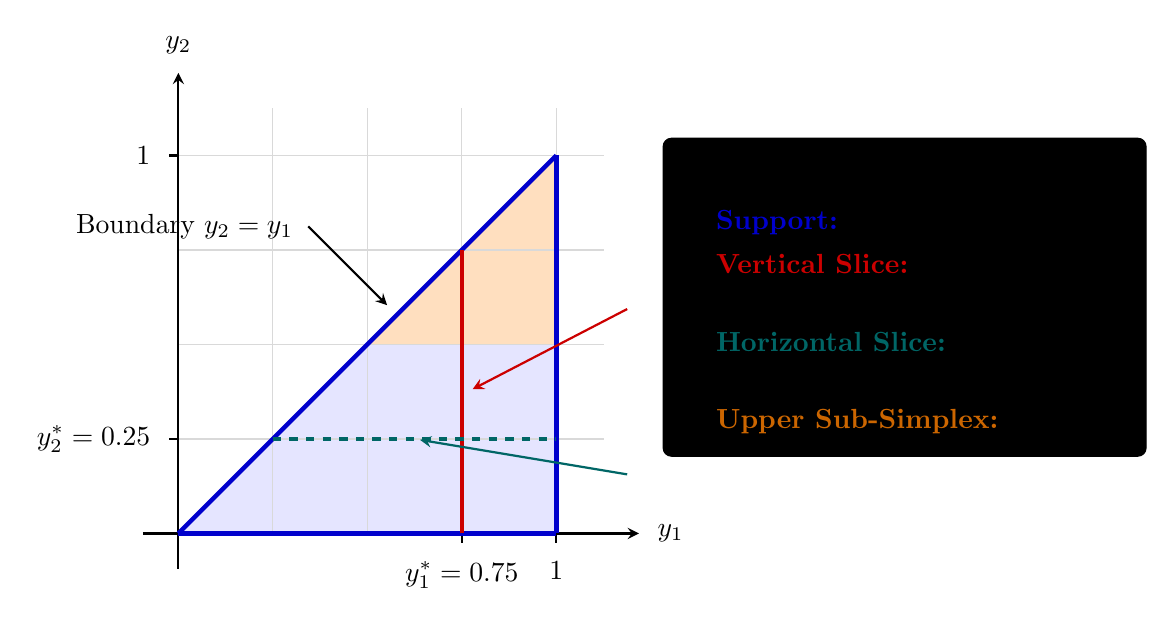
\begin{tikzpicture}[scale=1.5]
    % 1) \fill backgrounds
    \fill[blue!10] (0,0) -- (3.2,0) -- (3.2,3.2) -- cycle;
    \fill[orange!25] (1.6,1.6) -- (3.2,1.6) -- (3.2,3.2) -- cycle;

    % 2) \draw grid lines/axes
    \draw[gray!30, thin, step=0.8] (0,0) grid (3.6,3.6);
    \draw[->, >=stealth, thick, black] (-0.3,0) -- (3.9,0) node[right=3pt, black] {$\displaystyle y_1$};
    \draw[->, >=stealth, thick, black] (0,-0.3) -- (0,3.9) node[above=3pt, black] {$\displaystyle y_2$};

    % Tick marks
    \draw[thick, black] (3.2,0) -- (3.2,-0.08) node[below=3pt, black] {$\displaystyle 1$};
    \draw[thick, black] (0,3.2) -- (-0.08,3.2) node[left=3pt, black] {$\displaystyle 1$};
    \draw[thick, black] (2.4,0) -- (2.4,-0.08) node[below=3pt, black] {$\displaystyle y_1^* = 0.75$};
    \draw[thick, black] (0,0.8) -- (-0.08,0.8) node[left=3pt, black] {$\displaystyle y_2^* = 0.25$};

    % 3) \draw primary plots
    \draw[ultra thick, blue!80!black] (0,0) -- (3.2,3.2);
    \draw[ultra thick, blue!80!black] (3.2,0) -- (3.2,3.2);
    \draw[ultra thick, blue!80!black] (0,0) -- (3.2,0);

    % Conditional slices (fibers)
    \draw[ultra thick, red!80!black] (2.4,0) -- (2.4,2.4);
    \draw[ultra thick, teal!80!black, dashed] (0.8,0.8) -- (3.2,0.8);

    % 4) \node labels/text and callout arrows
    \draw[->, >=stealth, shorten >=2pt, thick, black] (1.1,2.6) -- (1.8,1.9);
    \node[above=3pt, left=2pt, black] at (1.1,2.6) {$\displaystyle \text{Boundary } y_2 = y_1$};

    \draw[->, >=stealth, shorten >=2pt, thick, red!80!black] (3.8,1.9) -- (2.45,1.2);
    \draw[->, >=stealth, shorten >=2pt, thick, teal!80!black] (3.8,0.5) -- (2.0,0.8);

    % Single-Node Multiline Legend using Anchor Pivot Strategy
    \node[draw=black, fill=white, rounded corners=3pt, align=left, inner sep=8pt, anchor=west, black] at (4.1, 2.0) {
        \textbf{Geometric Conditioning Guide}\\[6pt]
        $\displaystyle \blacksquare$ \textcolor{blue!80!black}{\textbf{Support:}} $\displaystyle \mathcal{S} = \{0 \le y_2 \le y_1 \le 1\}$\\[4pt]
        $\displaystyle \blacksquare$ \textcolor{red!80!black}{\textbf{Vertical Slice:}} $\displaystyle Y_1 = y_1^*$\\
        $\displaystyle \quad \implies y_2 \in [0,\ y_1^*]$\\[4pt]
        $\displaystyle \blacksquare$ \textcolor{teal!80!black}{\textbf{Horizontal Slice:}} $\displaystyle Y_2 = y_2^*$\\
        $\displaystyle \quad \implies y_1 \in [y_2^*,\ 1]$\\[4pt]
        $\displaystyle \blacksquare$ \textcolor{orange!80!black}{\textbf{Upper Sub-Simplex:}} $\displaystyle Y_2 \ge 0.5$
    };
\end{tikzpicture}
\end{center}

\vspace{0.4cm}

\begin{center}
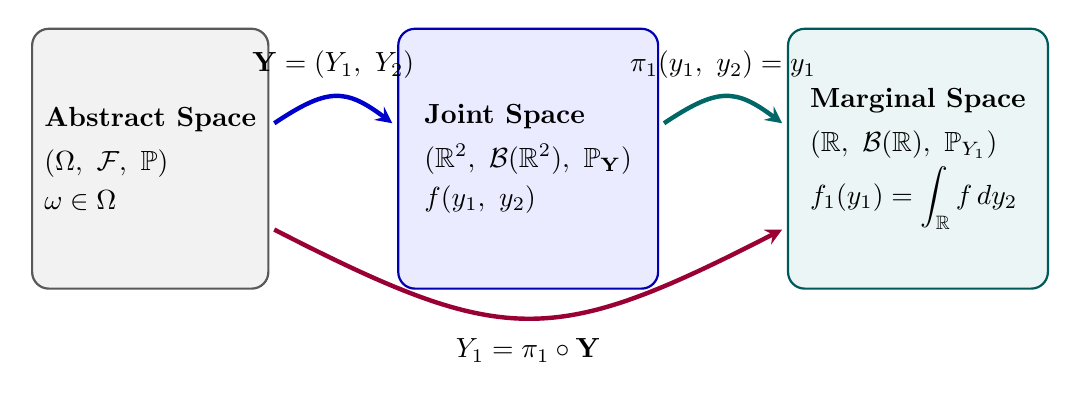
\begin{tikzpicture}[scale=1.5]
    % 1) \fill backgrounds
    \fill[gray!10, rounded corners=6pt] (-0.8,-0.6) rectangle (1.2,1.6);
    \fill[blue!8, rounded corners=6pt] (2.3,-0.6) rectangle (4.5,1.6);
    \fill[teal!8, rounded corners=6pt] (5.6,-0.6) rectangle (7.8,1.6);

    % 2) \draw borders of spaces
    \draw[thick, gray!70!black, rounded corners=6pt] (-0.8,-0.6) rectangle (1.2,1.6);
    \draw[thick, blue!70!black, rounded corners=6pt] (2.3,-0.6) rectangle (4.5,1.6);
    \draw[thick, teal!70!black, rounded corners=6pt] (5.6,-0.6) rectangle (7.8,1.6);

    % 3) \draw primary mapping arrows
    \draw[->, >=stealth, ultra thick, blue!80!black] (1.25, 0.8) .. controls (1.7, 1.1) and (1.85, 1.1) .. (2.25, 0.8);
    \draw[->, >=stealth, ultra thick, teal!80!black] (4.55, 0.8) .. controls (5.0, 1.1) and (5.15, 1.1) .. (5.55, 0.8);
    \draw[->, >=stealth, ultra thick, purple!80!black] (1.25, -0.1) .. controls (3.2, -1.1) and (3.6, -1.1) .. (5.55, -0.1);

    % 4) \node labels/text
    \node[align=left, inner sep=6pt, black] at (0.2, 0.5) {
        \textbf{Abstract Space}\\[4pt]
        $\displaystyle (\Omega,\ \F,\ \Prob)$\\[2pt]
        $\displaystyle \omega \in \Omega$
    };

    \node[align=left, inner sep=6pt, black] at (3.4, 0.5) {
        \textbf{Joint Space}\\[4pt]
        $\displaystyle (\mathbb{R}^2,\ \mathcal{B}(\mathbb{R}^2),\ \Prob_{\mathbf{Y}})$\\[2pt]
        $\displaystyle f(y_1,\ y_2)$
    };

    \node[align=left, inner sep=6pt, black] at (6.7, 0.5) {
        \textbf{Marginal Space}\\[4pt]
        $\displaystyle (\mathbb{R},\ \mathcal{B}(\mathbb{R}),\ \Prob_{Y_1})$\\[2pt]
        $\displaystyle f_1(y_1) = \int_{\mathbb{R}} f \, dy_2$
    };

    \node[above=4pt, black] at (1.75, 1.0) {$\displaystyle \mathbf{Y} = (Y_1,\ Y_2)$};
    \node[above=4pt, black] at (5.05, 1.0) {$\displaystyle \pi_1(y_1,\ y_2) = y_1$};
    \node[below=4pt, black] at (3.4, -0.85) {$\displaystyle Y_1 = \pi_1 \circ \mathbf{Y}$};
\end{tikzpicture}
\end{center}

\subsection{Heuristics and ``Cheats'' for Rapid Problem Solving}

\begin{enumerate}
    \item \textbf{The Support-First Rule for Independence:} Before computing a single marginal integral to check whether $Y_1$ and $Y_2$ are independent, inspect the \textbf{support} $\mathcal{S} = \{(y_1, y_2) : f(y_1, y_2) > 0\}$. If $\mathcal{S}$ is \textbf{not} a Cartesian product of univariate sets $A \times B$ (for example, if the boundary involves an inequality coupling $y_1$ and $y_2$, such as $0 \le y_1 \le y_2 \le 1$, $y_1 + y_2 \le 1$, or $y_1^2 + y_2^2 \le 1$), then $Y_1$ and $Y_2$ are \textbf{automatically dependent}! Only if $\mathcal{S} = A \times B$ do you need to check whether $f(y_1, y_2)$ factors into $g(y_1)h(y_2)$.
    \item \textbf{Proportionality Shortcut for Conditional Densities:} When computing $f(y_1 \mid y_2) = \frac{f(y_1, y_2)}{f_2(y_2)}$, remember that $y_2$ is held \textbf{constant}. Therefore, $f(y_1 \mid y_2) \propto_{y_1} f(y_1, y_2) \mathbf{1}_{\mathcal{S}(y_2)}(y_1)$. Any multiplicative factor depending only on $y_2$ will cancel out! For example, in Exercise 5.23, $f(y_1, y_2) = 3y_1$ on $0 \le y_2 \le y_1 \le 1$. Holding $y_1$ fixed, $f(y_2 \mid y_1)$ is constant with respect to $y_2$ on $[0, y_1]$, so $Y_2 \mid Y_1 = y_1$ \textit{must} be $\text{Uniform}(0, y_1)$ with density $1/y_1$—without even needing to compute $f_1(y_1)$ first!
    \item \textbf{Marginalizing Variable Limits:} When computing $f_1(y_1) = \int f(y_1, y_2) \, dy_2$, the variable $y_2$ is a dummy variable of integration. Consequently, $y_2$ can \textbf{never} appear in the final formula for $f_1(y_1)$ or in its support bounds; conversely, the limits of the integral with respect to $y_2$ may depend on $y_1$.
\end{enumerate}

\subsection{Common Pitfalls and Logical Fallacies}

\begin{itemize}
    \item \textbf{Pitfall 1: Forgetting the Support Indicator in Conditional Densities.} Writing $f(y_1 \mid y_2) = \frac{1}{y_2}$ without specifying $0 \le y_1 \le y_2$ is a major mathematical error. When integrating $f(y_1 \mid y_2)$ to find $\Prob(Y_1 \le a \mid Y_2 = y_2)$, the upper limit of integration is $\min(a, y_2)$, not $a$.
    \item \textbf{Pitfall 2: Confusing $\Prob(A \mid B)$ with $\Prob(B \mid A)$ (Prosecutor's / Base Rate Fallacy).} In Exercise 5.22, $\Prob(Y_2 = 2 \mid Y_1 = 0) = \frac{0.24}{0.76} \approx 0.3158$ (proportion of surviving children who used a car-seat belt) is completely different from $\Prob(Y_1 = 0 \mid Y_2 = 2) = \frac{0.24}{0.29} \approx 0.8276$ (survival probability given a car-seat belt was used).
    \item \textbf{Pitfall 3: Confusing Mutually Exclusive Events with Independent Events.} If $A$ and $B$ have positive probability and are mutually exclusive ($A \cap B = \emptyset$), then $\Prob(A \mid B) = 0 \neq \Prob(A)$, so they are maximally dependent.
    \item \textbf{Pitfall 4: Dividing by Zero Marginal Density.} The conditional density $f(y_1 \mid y_2)$ is undefined on the set $\{y_2 \in \mathbb{R} : f_2(y_2) = 0\}$. Always check boundary points (such as $y_2 = 1$ in Exercise 5.23(b), where $f_2(1) = \frac{3}{2}(1 - 1^2) = 0$).
\end{itemize}

\newpage
% ==============================================================================
% PART 5: CONCEPTUAL SYNTHESIS AND THE "BIG PICTURE"
% ==============================================================================
\section{Conceptual Synthesis and The ``Big Picture''}

\subsection{Thematic Connections: Disintegration and Projection of Measures}

The unifying mathematical theme of this chapter is the \textbf{decomposition and projection of product measures} (known in ergodic theory and abstract analysis as \textit{Rokhlin's Disintegration Theorem}). Across mathematics, whenever we study a high-dimensional object—whether a vector space in linear algebra, a fiber bundle in differential geometry, or a joint probability space $(\mathbb{R}^n, \mathcal{B}(\mathbb{R}^n), \Prob_{\mathbf{Y}})$—we understand its structure by decomposing it into:
\begin{enumerate}
    \item A \textbf{base space projection} (the marginal distribution $\Prob_{Y_2}$ on the base manifold), and
    \item A family of \textbf{fibers} over each point of the base space (the conditional distributions $\Prob_{Y_1 \mid Y_2 = y_2}$, which form a \textit{Markov kernel}).
\end{enumerate}
The multiplicative law $f(y_1, y_2) = f_2(y_2) f(y_1 \mid y_2)$ is the probabilistic incarnation of fiber bundle reconstruction: the total measure on the product space is reconstructed by integrating the fiber measures against the base measure:
\[ \Prob_{\mathbf{Y}}(dx_1 \times dx_2) = \Prob_{Y_1 \mid Y_2}(dx_1 \mid x_2) \, \Prob_{Y_2}(dx_2). \]
When the fiber measure $\Prob_{Y_1 \mid Y_2}(\cdot \mid x_2)$ is invariant with respect to the base point $x_2$, the bundle is trivial—which is the exact geometric meaning of \textbf{statistical independence} ($\Prob_{\mathbf{Y}} = \Prob_{Y_1} \otimes \Prob_{Y_2}$).

\subsection{Forward and Backward Links}

\begin{itemize}
    \item \textbf{Backward Links (Foundations):}
    Marginal and conditional distributions generalize Chapter 2's elementary set-based rules—the Law of Total Probability $\Prob(A) = \sum_i \Prob(A \mid B_i)\Prob(B_i)$, Bayes' Rule, and the multiplication rule $\Prob(A \cap B) = \Prob(A)\Prob(B \mid A)$—from discrete events to $\sigma$-algebras generated by continuous random variables. They also extend Chapter 3 and 4's univariate families (Binomial, Hypergeometric, Poisson, Uniform, Exponential, Gamma, Beta) into coupled multivariate systems.
    \item \textbf{Forward Links (Advanced Sequels):}
    \begin{enumerate}
        \item \textbf{Conditional Expectation and Martingales:} Integrating $y_1$ against $f(y_1 \mid y_2)$ yields the conditional expectation $\E[Y_1 \mid Y_2 = y_2]$, which is the minimum mean-squared error ($L^2$-orthogonal projection) predictor of $Y_1$ given $Y_2$. Extending $\sigma(Y_2)$ to a filtration $\{\F_t\}_{t \ge 0}$ defines \textbf{martingales} ($\E[M_t \mid \F_s] = M_s$ for $s < t$), the cornerstone of stochastic calculus.
        \item \textbf{Markov Processes and Chapman-Kolmogorov Equations:} A stochastic process $\{X_t\}_{t \ge 0}$ is Markov if its conditional distribution given the past depends only on the present state. Marginalizing out an intermediate state $X_s$ in the joint transition density yields the celebrated \textbf{Chapman-Kolmogorov Equation}:
        \[ f(x_t \mid x_r) = \int_{-\infty}^\infty f(x_t \mid x_s) f(x_s \mid x_r) \, dx_s \quad (r < s < t). \]
        \item \textbf{Bayesian Statistical Inference:} Exercises *5.41 and *5.42 are prototypes of hierarchical Bayesian modeling, where a parameter $\theta$ is endowed with a prior $f(\theta)$, combined with a likelihood $f(y \mid \theta)$ to form the marginal evidence $f(y) = \int f(y \mid \theta)f(\theta) \, d\theta$, and inverted to obtain the posterior $f(\theta \mid y) = \frac{f(y \mid \theta)f(\theta)}{f(y)}$.
    \end{enumerate}
\end{itemize}

\newpage
% ==============================================================================
% PART 6: ABSTRACT REAL-WORLD MODELING (AI, ML, & QUANT FINANCE)
% ==============================================================================
\section{Abstract Real-World Modeling (AI, ML, and Quantitative Finance)}

\subsection{Concrete Advanced Scenarios}

\begin{enumerate}
    \item \textbf{Generative AI — Score-Based Diffusion Models and Variational Autoencoders (VAEs):}
    Modern generative AI models (such as Stable Diffusion and Sora) aim to sample from a complex, high-dimensional marginal data distribution $f_{\mathbf{X}_0}(\mathbf{x}_0)$ (e.g., natural images). Because $f_{\mathbf{X}_0}(\mathbf{x}_0)$ is intractable directly, a forward stochastic process progressively corrupts $\mathbf{X}_0$ with Gaussian noise via a known conditional transition density $f(\mathbf{x}_t \mid \mathbf{x}_0) = \mathcal{N}(\mathbf{x}_t; \sqrt{\bar{\alpha}_t}\mathbf{x}_0, (1 - \bar{\alpha}_t)\mathbf{I})$. Generation is achieved by learning the reverse-time conditional distribution $f(\mathbf{x}_{t-1} \mid \mathbf{x}_t)$, which is governed by the score of the marginal density $\nabla_{\mathbf{x}_t} \ln f_t(\mathbf{x}_t) = \nabla_{\mathbf{x}_t} \ln \int f(\mathbf{x}_t \mid \mathbf{x}_0) f_{\mathbf{X}_0}(\mathbf{x}_0) \, d\mathbf{x}_0$.
    \item \textbf{Quantitative Finance — Derivative Pricing and the Breeden-Litzenberger Formula:}
    In arbitrage-free option pricing under a risk-neutral probability measure $\mathbb{Q}$, the price at time $t$ of a European contingent claim with payoff $g(S_T)$ at maturity $T$ given current asset price $S_t = s$ is a conditional expectation integrated against the conditional risk-neutral transition density $f^{\mathbb{Q}}(s_T \mid S_t = s)$:
    \[ V(t, s) = e^{-r(T - t)} \E^{\mathbb{Q}}[g(S_T) \mid S_t = s] = e^{-r(T - t)} \int_0^\infty g(s_T) f^{\mathbb{Q}}(s_T \mid S_t = s) \, ds_T. \]
    In credit risk modeling (e.g., Gaussian and Student-$t$ copula CDO pricing), default times $(Y_1, Y_2)$ of correlated obligors are modeled exactly like Exercise 5.18 and Exercise *5.42 via conditional independence given a latent macroeconomic factor $\Lambda$.
    \item \textbf{Algorithmic Trading \& Stochastic Filtering — Kalman-Bucy and Particle Filtering:}
    In high-frequency statistical arbitrage, the true fundamental spread $Y_{1,t}$ of a cointegrated pair of assets is an unobserved latent state, while market microstructure noise produces noisy order-book observations $Y_{2,t}$. At each tick, the trading algorithm computes the marginal predictive density $f(y_{1,t} \mid \F_{t-1}) = \int f(y_{1,t} \mid y_{1,t-1}) f(y_{1,t-1} \mid \F_{t-1}) \, dy_{1,t-1}$ and updates to the conditional filtering density $f(y_{1,t} \mid \F_t)$ via continuous Bayes' Theorem.
\end{enumerate}

\subsection{Rigorous Quantitative Model Setup: Latent-Factor Variational Inference and Stochastic Filtering}

We formulate a rigorous mathematical framework unifying \textbf{Variational Autoencoders (VAEs)} in Machine Learning and \textbf{Continuous-Time Stochastic Filtering} in Quantitative Finance.

\textbf{1. Probability Space and Latent-Observation State Space:}
Let $(\Omega, \F, \Prob)$ be a complete probability space. Let $\mathbf{Z} \in \mathbb{R}^d$ be an unobserved latent state vector (representing latent semantic features in a generative model or unobserved stochastic volatility/drift factors in finance) and $\mathbf{X} \in \mathbb{R}^m$ be an observable data vector. Assume $(\mathbf{X}, \mathbf{Z})$ admits a strictly positive joint density $f(\mathbf{x}, \mathbf{z})$ with respect to Lebesgue measure $\lambda_{m+d}$ on $\mathbb{R}^m \times \mathbb{R}^d$, factored via Definition 5.7 as:
\[ f_\theta(\mathbf{x}, \mathbf{z}) = p_\theta(\mathbf{z}) \, p_\theta(\mathbf{x} \mid \mathbf{z}), \]
where $p_\theta(\mathbf{z})$ is the prior marginal density of $\mathbf{Z}$, $p_\theta(\mathbf{x} \mid \mathbf{z})$ is the conditional likelihood decoder parameterized by $\theta \in \Theta$, and the marginal data density (model evidence) is:
\[ p_\theta(\mathbf{x}) = \int_{\mathbb{R}^d} p_\theta(\mathbf{x}, \mathbf{z}) \, d\mathbf{z} = \int_{\mathbb{R}^d} p_\theta(\mathbf{x} \mid \mathbf{z}) p_\theta(\mathbf{z}) \, d\mathbf{z}. \]

\textbf{2. Intractability of the True Posterior and Variational Optimization Problem:}
By Definition 5.7, the exact conditional posterior density is $p_\theta(\mathbf{z} \mid \mathbf{x}) = \frac{p_\theta(\mathbf{x}, \mathbf{z})}{p_\theta(\mathbf{x})}$. Because the marginal integral $p_\theta(\mathbf{x})$ is analytically intractable in high dimensions $d \gg 1$, we introduce a tractable family of variational conditional densities $q_\phi(\mathbf{z} \mid \mathbf{x})$ parameterized by $\phi \in \Phi$.

\begin{proposition}[Evidence Lower Bound (ELBO) Decomposition]
For any observation $\mathbf{x} \in \mathbb{R}^m$ with $p_\theta(\mathbf{x}) > 0$, the log-marginal density satisfies the identity:
\[ \ln p_\theta(\mathbf{x}) = \mathcal{L}_{\text{ELBO}}(\theta, \phi; \mathbf{x}) + D_{\text{KL}}\left( q_\phi(\mathbf{z} \mid \mathbf{x}) \;\|\; p_\theta(\mathbf{z} \mid \mathbf{x}) \right), \]
where the Kullback-Leibler divergence is $D_{\text{KL}}(q \| p) = \int_{\mathbb{R}^d} q_\phi(\mathbf{z} \mid \mathbf{x}) \ln \frac{q_\phi(\mathbf{z} \mid \mathbf{x})}{p_\theta(\mathbf{z} \mid \mathbf{x})} \, d\mathbf{z} \ge 0$, and the Evidence Lower Bound is:
\[ \mathcal{L}_{\text{ELBO}}(\theta, \phi; \mathbf{x}) = \E_{q_\phi(\mathbf{z} \mid \mathbf{x})}\left[ \ln p_\theta(\mathbf{x} \mid \mathbf{z}) \right] - D_{\text{KL}}\left( q_\phi(\mathbf{z} \mid \mathbf{x}) \;\|\; p_\theta(\mathbf{z}) \right). \]
\end{proposition}

\begin{proof}
Since $\int_{\mathbb{R}^d} q_\phi(\mathbf{z} \mid \mathbf{x}) \, d\mathbf{z} = 1$ and $p_\theta(\mathbf{x}, \mathbf{z}) = p_\theta(\mathbf{x}) p_\theta(\mathbf{z} \mid \mathbf{x})$ by Definition 5.7:
\begin{align*}
    \ln p_\theta(\mathbf{x}) &= \int_{\mathbb{R}^d} q_\phi(\mathbf{z} \mid \mathbf{x}) \ln p_\theta(\mathbf{x}) \, d\mathbf{z} = \int_{\mathbb{R}^d} q_\phi(\mathbf{z} \mid \mathbf{x}) \ln \left( \frac{p_\theta(\mathbf{x}, \mathbf{z})}{p_\theta(\mathbf{z} \mid \mathbf{x})} \frac{q_\phi(\mathbf{z} \mid \mathbf{x})}{q_\phi(\mathbf{z} \mid \mathbf{x})} \right) d\mathbf{z} \\
    &= \int_{\mathbb{R}^d} q_\phi(\mathbf{z} \mid \mathbf{x}) \ln \left( \frac{p_\theta(\mathbf{x} \mid \mathbf{z}) p_\theta(\mathbf{z})}{q_\phi(\mathbf{z} \mid \mathbf{x})} \right) d\mathbf{z} + \int_{\mathbb{R}^d} q_\phi(\mathbf{z} \mid \mathbf{x}) \ln \left( \frac{q_\phi(\mathbf{z} \mid \mathbf{x})}{p_\theta(\mathbf{z} \mid \mathbf{x})} \right) d\mathbf{z} \\
    &= \mathcal{L}_{\text{ELBO}}(\theta, \phi; \mathbf{x}) + D_{\text{KL}}\left( q_\phi(\mathbf{z} \mid \mathbf{x}) \;\|\; p_\theta(\mathbf{z} \mid \mathbf{x}) \right).
\end{align*}
By Jensen's inequality, $D_{\text{KL}}(q_\phi \| p_\theta) \ge 0$, with equality if and only if $q_\phi(\mathbf{z} \mid \mathbf{x}) = p_\theta(\mathbf{z} \mid \mathbf{x})$ almost everywhere.
\end{proof}

\textbf{3. Continuous-Time Stochastic Differential Equation (SDE) Extension (Fokker-Planck Marginal Evolution):}
In quantitative finance, if the state $Y_t \in \mathbb{R}$ evolves according to the It\^o SDE
\[ dY_t = \mu(t, Y_t) \, dt + \sigma(t, Y_t) \, dW_t, \qquad Y_0 = y_0, \]
where $W_t$ is a standard Brownian motion, then by It\^o's Lemma and integration by parts against compactly supported test functions, the conditional transition density $f(y, t \mid y_0, 0)$ satisfies the \textbf{Forward Kolmogorov (Fokker-Planck) Partial Differential Equation}:
\[ \frac{\partial}{\partial t} f(y, t \mid y_0, 0) = -\frac{\partial}{\partial y}\Big[ \mu(t, y) f(y, t \mid y_0, 0) \Big] + \frac{1}{2} \frac{\partial^2}{\partial y^2}\Big[ \sigma^2(t, y) f(y, t \mid y_0, 0) \Big]. \]

\newpage
% ==============================================================================
% PART 7: COMMON VARIATIONS AND UNTESTED CONCEPTS
% ==============================================================================
\section{Common Variations and Untested Concepts}

Standard university examinations on Marginal and Conditional Probability Distributions frequently test three advanced theoretical variations not directly covered in Exercises 5.15--5.42:
\begin{enumerate}
    \item \textbf{The Bivariate Normal Distribution and Exact Gaussian Conditioning.}
    \item \textbf{Hammerstein's Counterexample: Pairwise / Marginal Normality Does Not Imply Joint Normality.}
    \item \textbf{Borel's Paradox and Coordinate-Dependence of Conditioning on Measure-Zero Manifolds.}
\end{enumerate}

\subsection{Variation 1: Conditional Distribution of the Bivariate Normal Law}

\begin{theorem}[Bivariate Normal Marginals and Conditionals]
Let $(Y_1, Y_2)$ have the Bivariate Normal joint density with parameters $(\mu_1, \mu_2, \sigma_1^2, \sigma_2^2, \rho)$, where $\sigma_1, \sigma_2 > 0$ and $\rho \in (-1, 1)$:
\[ f(y_1, y_2) = \frac{1}{2\pi \sigma_1 \sigma_2 \sqrt{1 - \rho^2}} \exp\left( -\frac{1}{2(1 - \rho^2)} \left[ z_1^2 - 2\rho z_1 z_2 + z_2^2 \right] \right), \quad z_i = \frac{y_i - \mu_i}{\sigma_i}. \]
Then:
\begin{enumerate}[label=(\alph*)]
    \item The marginal distributions are $Y_1 \sim \mathcal{N}(\mu_1, \sigma_1^2)$ and $Y_2 \sim \mathcal{N}(\mu_2, \sigma_2^2)$.
    \item The conditional distribution of $Y_1$ given $Y_2 = y_2$ is Normal:
    \[ Y_1 \mid Y_2 = y_2 \sim \mathcal{N}\left( \mu_1 + \rho \frac{\sigma_1}{\sigma_2}(y_2 - \mu_2), \; \sigma_1^2(1 - \rho^2) \right). \]
\end{enumerate}
\end{theorem}

\begin{proof}
We complete the square in $z_1$ inside the quadratic form $Q(z_1, z_2) = z_1^2 - 2\rho z_1 z_2 + z_2^2$:
\[ Q(z_1, z_2) = (z_1 - \rho z_2)^2 + (1 - \rho^2)z_2^2 = (1 - \rho^2)z_2^2 + \left( \frac{y_1 - \left[\mu_1 + \rho \frac{\sigma_1}{\sigma_2}(y_2 - \mu_2)\right]}{\sigma_1} \right)^2. \]
Substituting this decomposition into $f(y_1, y_2)$ factors the joint density directly into $f_2(y_2) \cdot f(y_1 \mid y_2)$:
\[ f(y_1, y_2) = \underbrace{\left[ \frac{1}{\sqrt{2\pi}\sigma_2} \exp\left( -\frac{(y_2 - \mu_2)^2}{2\sigma_2^2} \right) \right]}_{f_2(y_2)} \cdot \underbrace{\left[ \frac{1}{\sqrt{2\pi}\sigma_1\sqrt{1-\rho^2}} \exp\left( -\frac{\left(y_1 - \left[\mu_1 + \rho\frac{\sigma_1}{\sigma_2}(y_2 - \mu_2)\right]\right)^2}{2\sigma_1^2(1 - \rho^2)} \right) \right]}_{f(y_1 \mid y_2)}. \]
Integrating with respect to $y_1 \in (-\infty, \infty)$ integrates the second factor (a Gaussian density in $y_1$) to $1$, leaving $f_2(y_2) = \mathcal{N}(y_2; \mu_2, \sigma_2^2)$. Dividing $f(y_1, y_2)$ by $f_2(y_2)$ immediately isolates $f(y_1 \mid y_2)$ as a Normal density with conditional mean $\mu_{Y_1 \mid y_2} = \mu_1 + \rho \frac{\sigma_1}{\sigma_2}(y_2 - \mu_2)$ and reduced conditional variance $\sigma_{Y_1 \mid y_2}^2 = \sigma_1^2(1 - \rho^2)$.
\end{proof}

\subsection{Variation 2: Marginal Distributions Do Not Uniquely Determine the Joint Distribution}

\begin{example}[Non-Gaussian Joint Density with Standard Normal Marginals]
Prove that the bivariate function
\[ f(y_1, y_2) = \frac{1}{\pi} \exp\left( -\frac{1}{2}(y_1^2 + y_2^2) \right) \mathbf{1}_{\{y_1 y_2 \ge 0\}}(y_1, y_2), \quad (y_1, y_2) \in \mathbb{R}^2, \]
is a valid joint probability density whose marginal distributions are both Standard Normal ($Y_1



\end{document}